% !TEX TS-program = xelatex
% !BIB TS-program = bibtex
\documentclass[12pt,letterpaper]{article}
\usepackage{style/dsc180reportstyle} % import dsc180reportstyle.sty
\usepackage{wasysym}
\usepackage{subcaption}
\newcommand{\ind}{\perp\!\!\!\!\perp}
\SetKwComment{Comment}{/* }{ */}

\def\multimapboth{\kern2pt\hbox{$\circ$}\kern-1pt\hbox{$-$}\kern-1pt\hbox{$\circ$}\kern2pt}
\def\circrightarrow{\kern2pt\hbox{$\circ$}\kern-1.5pt\hbox{$\to$}\kern2pt}
\def\circleftarrow{\kern2pt\hbox{$\leftarrow$}\kern-1.5pt\hbox{$\circ$}\kern2pt}

%%%%%%%%%%%%%%%%%%%%%%%%%%%%%%%%%%%%%%%%%%%%%%%%%%%%%%%%
%%%% Title and Authors
%%%%%%%%%%%%%%%%%%%%%%%%%%%%%%%%%%%%%%%%%%%%%%%%%%%%%%%%

\title{Causal Discovery in Gut Microbes for PCOS}

\author{Mariana Paco Mendivil \\
  {\tt mpacomendivil@ucsd.edu} \\\And
  Candus Shi \\
  {\tt c6shi@ucsd.edu} \\\And
  Nicole Zhang \\
  {\tt nwzhang@ucsd.edu} \\\And
  Biwei Huang \\
  {\tt bih007@ucsd.edu} \\\And
  Jelena Bradic \\
  {\tt jbradic@ucsd.edu}}

\begin{document}
\maketitle

%%%%%%%%%%%%%%%%%%%%%%%%%%%%%%%%%%%%%%%%%%%%%%%%%%%%%%%%
%%%% Abstract and Links
%%%%%%%%%%%%%%%%%%%%%%%%%%%%%%%%%%%%%%%%%%%%%%%%%%%%%%%%


\begin{abstract}
    \textcolor{black}{
    The human gut microbiome has become a significant factor in understanding metabolic health, influencing conditions such as type 2 diabetes (T2D) and polycystic ovary syndrome (PCOS). Despite its recognized impact, much of the current research on the human gut microbiome and diseases remain limited to associative and correlational studies, leaving gaps in understanding the underlying causal relationships. This study addresses these gaps by utilizing causal discovery algorithms and causal inference methods and comparing them with prediction models to investigate microbial contributions to T2D and PCOS. First, we graph the microbe-microbe interaction networks on the genus level for healthy and diseased cohorts using a version of the Peter-Clark (PC) algorithm altered to reduce the multiple testing burden. Then, we graph the microbe-disease interaction network on the genus level for a disease using the constraint-based causal discovery from heterogeneous/nonstationary data algorithm (CD-NOD) and compare the microbes directly linked to disease with microbes from a variational autoencoder (VAE) prediction model. Our results show that \textit{Butyricimonas, Clostridium XIVb, Odoribacter, unclassified Bacteria}, and \textit{unclassified Firmicutes} are causal to T2D; \textit{Alistipes, Blautia, Burkholderia, Desulfovibrio, Holdemanella, Knoellia, Prevotellaceae NK3B31, Ruminococcus}, and \textit{Ruminococcus gnavus} are causal to PCOS. Finally, we compute their causal effects using do-calculus and compare with the differential analysis method BIRDMAn. This work aims to provide a framework for investigating causal relationships between the gut microbiome and other diseases as well as guide further research and wet-lab experiments and develop a stronger understanding of the role of the gut microbiome in precision medicine.}
\end{abstract}

\begin{center}
Code: \url{https://github.com/nzhang20/Causal-Discovery-on-Gut-Microbial-Data-for-Disease-Risk-Prediction}
\end{center}

\maketoc
\clearpage

%%%%%%%%%%%%%%%%%%%%%%%%%%%%%%%%%%%%%%%%%%%%%%%%%%%%%%%%
%%%% Main Contents
%%%%%%%%%%%%%%%%%%%%%%%%%%%%%%%%%%%%%%%%%%%%%%%%%%%%%%%%

\section{Introduction}

The human gut microbiome has gained significant attention in recent years for its important role in metabolic health. While there has been extensive research that links the microbiome to health disorders such as type 2 diabetes (T2D) \citep{zhou2019t2d} and polycystic ovary syndrome (PCOS) \citep{yang2024pcos}, the majority of these studies remain correlational, leaving causal relationships undiscovered. Understanding these relationships is essential to improving and personalizing medical treatments for such diseases.
This study builds on recent advancements in causal discovery algorithms to investigate how microbial taxa influence metabolic disorders. Our goal is to find patterns that conventional association-based methods might miss by leveraging the marginal and conditional independencies found in the data as well as graph theory to assess where a causal relationship might occur and if possible, its causal direction. Given the high-dimensional nature of this type of data, we also explore different feature pruning techniques to reduce the multiple testing burden and for ease of interpretation. 

We focus on two aspects of causal discovery and causal inference in the gut microbiome. First, we are curious to see how the microbe-microbe interaction networks may differ between the two outcome groups. Due to the high number of features compared to the number of samples in gut microbiome abundance data, we first reduce the number of edges between microbes using a sparse correlation method, SparCC \citep{weiss2016correlationbenchmark, friedman2012sparcc}, and a sparse precision matrix estimator, graphical lasso \citep{friedman2008glasso}. Then, we graph the two networks for the corresponding cohorts using a constraint-based causal discovery algorithm similar to the Peter-Clark (PC) algorithm \citep{glymour2019review}, but with a smaller depth and without a direction orientation step to reduce the multiple testing burden.

Second, we are also interested in graphing the microbe-disease interaction network, where we are particularly interested in the microbes directly linked to disease status. Instead of reducing the number of edges, we reduce the number of features using logistic lasso regression to account for the relationships of microbes to the outcome variable. Finally, we graph the network using the features that survive lasso and a disease status node using the constraint-based causal discovery from heterogeneous/nonstationary data algorithm (CD-NOD) \citep{huang2019cdnod} to identify microbes directly linked to disease status. Given the predictive nature of graphing a microbe-disease interaction network, we are also interested in developing a prediction model for disease using a causal representation learning technique embedding each sample with a Variational Autoencoder (VAE) in a classification task \citep{khemakhem2020vaenonlinearica}, then comparing the results from CD-NOD to the microbes used in the model.

After obtaining the causal structure from CD-NOD, we move to the causal inference stage of our analysis. We use a variety of causal inference methods such as do-calculus and doubly robust estimation to estimate the causal effect of a microbe on disease status. We compare these results with a differential analysis method that also accounts for heterogeneity in the data, Bayesian Inferential Regression for Differential Microbiome Analysis (BIRDMAn) \citep{rahman2023birdman}. 

\subsection{Literature Review}

\textbf{T2D}

T2D is a metabolic disease where individuals have chronic high blood sugar, otherwise known as hyperglycaemia. This is a result of insulin resistance where the pancreas produces insulin, but the cells do not respond to it, leading the pancreas to try to produce more insulin. The pancreas eventually fails to keep producing insulin leading to low insulin levels and high blood sugar, and this can lead to increased risks of developing other diseases such as heart disease and kidney disease \citep{adat2d}. T2D affects millions of people, and many studies have been conducted to investigate its underlying cause, its common precursor coined as “prediabetes”, and other factors that can contribute or affect the development of T2D \citep{tabak2012prediabetes, qin2012mgwast2d, mehta2000hcvt2d}. 

Given the impactful role of the gut microbiome on human health, numerous studies have also investigated the relationship between gut microbiota and T2D. For example, \citep{zhou2019t2d} conducted a longitudinal study of multi-omic data on healthy individuals vs individuals with prediabetes (an early stage of T2D) to determine how microbes behave differently between the two cohorts. They found that variation in microbes between and within individuals of each cohort differed, that each cohort responded to infections and immunizations differently, and through associations, that host-microbe interactions differed between the two cohorts. In particular, they found that “the genus \textit{Holdemania} was significantly associated with \textit{Clostridium XIVb} and \textit{Phascolarctobacterium} in insulin-sensitive participants, but significantly correlated with \textit{Clostridium XIVa}, \textit{Clostridium XVII}, \textit{Collinsella}, \textit{Lachnospiracea incertae sedis}, and \textit{unclassified Lachnospiraceae} in insulin-resistant participants”. \citep{baars2024gutt2d} also found common results from various studies investigating this relationship: there appears to be “a reduction of butyrate-producing bacteria such as \textit{Faecalibacterium}, \textit{Clostridium}, and \textit{Akkermansia} in individuals with T2D”. 

These analyses demonstrate that there are significant differences in microbe interactions between healthy and prediabetic individuals, and furthermore, that we can discover the causal graph from their data and use causality to determine which host-microbe interactions this study found through associations are not spurious, but causal. \newline

\textbf{PCOS}

PCOS is a complex endocrine disorder linked to metabolic diseases such as obesity and T2D. It affects 6-13\% of women of reproductive age, and 70\% of affected women remain undiagnosed as the causes of PCOS largely remains a mystery \citep{who2025pcos}. In fact, it was not until quite recently that the scientific community has peaked interest in studying PCOS and its causes. Current diagnostic methods use hormone and metabolic biomarkers, but these techniques are insufficient to differentiate between different PCOS subtypes, such as those characterized by hyperandrogenism. Due to inconsistent study findings, regional differences, and heterogeneity in studies, the association between PCOS and gut microbiota is not well-defined. \citep{yang2024pcos} conduct an individual participant data meta-analysis and systematic review to see if gut microbiota characteristics between healthy individuals and PCOS patients, between different subtypes of PCOS, and regional differences can be identified using data from a variety of clinical trials.

Using Wilcoxon tests with Benjamini-Hochberg corrected p-values, they found differential bacteria between the healthy and PCOS groups: PCOS patients had slightly lower levels of \textit{Bacillota} and higher levels of \textit{Actinobacteriota}; PCOS patients in China had lower alpha diversity than healthy controls, whereas PCOS patients in Europe had higher diversity; PCOS patients with high testosterone (HT) had different microbial patterns compared to those with low testosterone (LT), including lower levels of \textit{Faecalibacterium} and higher levels of \textit{Prevotella}. 

With biomarkers like \textit{Faecalibacterium} and \textit{Prevotella}, PCOS subtypes have distinct gut microbiota compositions that are impacted by geography and testosterone levels. These results highlight the possibility of personalized treatments based on microbiota. However, to handle population variety and improve strain-level assessments, extensive, global research is required. Given this complexity, we are interested in identifying potential biomarkers for all types of PCOS, i.e. disregarding the hyperandrogenism subtypes. \newline

\textbf{Gut Microbiome Analysis}

A typical gut microbiome analysis pipeline involves an upstream component and a downstream component. The upstream analysis typically starts with the raw sequencing files and involves demultiplexing, denoising, and classification to determine which OTUs are present and their abundance. There are multiple methods with their own unique advantages and disadvantages. The most common method is 16s rRNA sequencing which is a type of amplicon analysis, and amplifies a piece of DNA that occurs within the 16s rRNA PCR primer region, and based on a region of the 16s rRNA gene (V1-V9), can differentiate bacterial taxa \citep{allaband2019microbiome101}. Then, one can try to identify the taxa by placing the sequences onto a phylogenetic tree or matching them to a taxonomy database. There are also different databases that have been curated such as Greengenes2 \citep{mcdonald2024greengenes2}, SILVA \citep{pruesse2007silva}, and RDP \citep{cole2014rdp}, and the choice of database can also affect results. These databases are also often highly incomplete, making this taxonomy-identification task quite difficult and sensitive to choice of parameters. 

Besides 16s rRNA sequencing, shotgun metagenomics is another method gaining traction for its ability to infer a complete list of microbial strains, fungi, and viruses (which are different from bacteria), which are missed by 16s rRNA. It works by sequencing small fragments of the DNA and trying to piece them back together into a view of the microbiome, rather than only looking at one gene like 16s rRNA. However, since it uses more than one gene, it is limited by the number of unknown microbe genomes. As more researchers work on studying the gut microbiome, we can expect this issue to diminish as we uncover more microbe genomes. 

The downstream analysis then proceeds with the abundance table to analyze differences in microbiome composition between groups, also known as differential analysis, and calculate different measures of diversity. For example, alpha diversity is a measure of intra-subject variability, while beta diversity measures inter-subject variability, and each diversity measure has different metrics such Chao1, Shannon, Faith’s phylogenetic diversity for alpha diversity, and Bray-Curtis, Jaccard, and UniFrac for beta diversity \citep{knight2018bestpractices}. Current differential analysis methods include applying an isometric log-ratio transformation to account for the compositionality of the data, then proceeding with standard regression and classification models. \newline

\textbf{Causal Discovery and the Gut Microbiome}

There have been previous attempts to perform causal discovery on the gut microbiome. In particular, \citep{sazal2021causalgut} attempts to use causal discovery to construct causal networks and implement do-calculus, a causal inference technique developed by \citep{pearl2016primer} to estimate the causal effects of microbes on other microbes and on outcome variables. For the causal discovery task, they use the PC-stable algorithm \citep{colombo2014pcstable} which is a variation of PC that removes order-dependence during the estimation of the skeleton of the casual graph. The advantage of PC-stable over PC is that PC may output different results given the order of the conditional independence tests done. After finding the causal graphs, they used do-calculus to quantify the effects of each edge in the graphs which essentially uses the do-operator to intervene on the treatment node, remove all edges pointing towards said node, and to estimate the interventional expectation of the outcome node using a model appropriate for the given data structure like linear regression. They test their pipeline’s consistency using simulations and apply their pipeline to real dataset of healthy individuals, individuals with ulcerative colitis (UC), and individuals with Crohn’s disease (CD). They used bootstraps to compute confidence intervals for each edge and permutation tests to calculate p-values for the overall network and found bacteria beneficial to UC such as \textit{unclassified Oscillibacter}, \textit{Sutterella wadsworthensis}, and \textit{Bacteroides xylanisolvens}. However, they fail to account for multiple testing issues and covariates in their networks. Since we designed our study before finding this paper, we see a promising role of causal discovery and causal inference in gut microbial data for studying various human diseases. 

Additionally, there have been advancement to causal discovery algorithms since the development of the PC and PC-stable algorithms. For example, a variant of the PC algorithm, CD-NOD \citep{huang2019cdnod}, was developed specifically for heterogeneous data, where the heterogeneity of the observed data can help discover the causal structure given certain variables that can change the distribution of the data. This is particularly useful with gut microbiome data where a dataset may contain samples from different studies, hence providing a heterogeneous dataset where the study ID can change the data distribution. 

\subsection{Data}

To answer our research question, we used the NIH Human Microbiome Project (HMP2) dataset \citep{zhou2019t2d} for T2D and the aggregated dataset from an individual participant data (IPD) meta analysis and systematic review conducted by \citep{yang2024pcos} for PCOS. We also conducted a meta-analysis of T2D studies to enhance the diversity of the study regions. The corresponding metadata can be found in the Appendix.

The HMP2 dataset \citep{zhou2019t2d} followed 106 participants for up to four years, collecting blood, stool, and nasal samples at every self-reported healthy visit and additional visits during periods of respiratory viral infection (RVI), influenza immunization, and other stresses such as antibiotic treatment. Since we are interested in the gut microbes, we look specifically at the visits where gut microbial taxa were profiled using 16S sequencing which provides normalized gut microbe abundance for taxa classified at 6 phyla, 28 classes, 12 orders, 21 families, and 45 genera. As the study authors illustrate, the gut microbiome can fluctuate with the presence of antibiotics and other stressor events such as illness, so we also only look at the visits that were classified as “Healthy”. For each individual, there is information about their race, sex, age, BMI, steady-state plasma glucose (SSPG), and insulin sensitivity classification. For 66 participants, their insulin sensitivity was assessed using an insulin suppression test measured by SSPG: 31 individuals were insulin-sensitive (IS: SSPG < 150 mg/dl), and 35 individuals were insulin-resistant (IR: SSPG $\geq$150 mg/dl). The remaining 40 individuals are classified as unknown due to medical contraindications leading to a lack of insulin suppression tests. Since the dataset is longitudinal but with very few time points per subject, we treated it as a cross-sectional dataset, leaving us with 153 and 178 samples for the IS and IR cohorts respectively.

The IPD meta analysis dataset \citep{yang2024pcos} is an aggregation of the 14 studies that were included in the systematic review, but at the individual level. This is different from a meta analysis which analyzes aggregated data or statistics from multiple different studies. Each row of this PCOS dataset represents one sample of gut microbe abundance measurements as well as the sample’s study’s region (Asia or Europe), the sample’s classification as a PCOS patient or a healthy control (HC), and if they were a PCOS patient, whether they had low (LT) or high (HT) testosterone levels. This granularity gives us more data and statistical power behind our results rather than using just one PCOS study. Since the only considerations for confounding their selection criteria specified were no drug interventions, there are other gut microbiome-related confounders that may be present in our data, such as diet, alcohol usage, stress, etc. We examined the study designs of the 14 included studies and found that they varied in external factors including diet, alcohol consumption, the use of antibiotics, and more. Although this is a limitation with the dataset, we chose to continue with this dataset due to its large sample size. This dataset provided us with 1,128 genera and 435 HC \& 513 PCOS individuals. 

For the T2D meta-analysis, we chose 7 studies, with 284 non-T2D and 527 T2D individuals from Japan, Indonesia, Pakistan, Vietnam, Finland, and Sudan. They are all V3-V4 primer regions, adult samples, and use 16s rRNA sequencing.

\section{Methods}

In this study, we use causal discovery algorithms and compare them with predictive modeling to explore the causal relationships between the gut microbiome and two diseases: T2D and PCOS. We used datasets that were cross-sectional, meaning they provide a snapshot of the gut microbiome and disease status at a single point in time, which makes it challenging to determine whether changes in the microbiome cause the disease or are a result of it. Rather than recovering this information from experiments that can be expensive, we can use computational methods to discover causality to the best of the data’s ability. 

Our approach tackles the complexities of working with high-dimensional data (many microbial features) and relatively small sample sizes. We use feature selection and sure screening techniques to reduce the dimensions of these datasets, and we adjust existing causal discovery algorithms to reduce the multiple testing burden. The goal is to build a framework for understanding how gut microbes contribute to disease and to identify potential targets for personalized treatments.  

\subsection{Data Preprocessing}

For the T2D dataset we removed subjects with an unknown insulin resistance status and selecting only the “Healthy” sample visits. We extracted microbial abundance data at the genus level and converted the values to percentages. The dataset was then merged across subject, sample, and microbial abundance files, with categorical variables like disease status (IRIS), gender, and ethnicity encoded numerically.

For the PCOS dataset, we grouped any unclassified microbial data into a single category and numerically encoded binary variables such as region, and disease status. To account for differences in the study sites, we created a study site variable by manually comparing the study sample sizes and regions.

Based on the suggestions provided by \citep{weiss2016correlationbenchmark} on different correlation strategies to use for different structures of a gut microbe dataset, we filtered out rare operational taxonomy units (OTUs), using a rareness threshold of 1\%. This helped reduce features substantially for the PCOS dataset from 1,128 genera to 274 genera. 

\subsection{Feature Selection and Sure Screening}

Given the high-dimensional nature of the PCOS dataset, we experimented with different feature selection and sure screening methods to reduce the feature space before running causal discovery algorithms to reduce the multiple testing burden on the causal discovery algorithms. The two tasks at hand call for different methods. For the microbe-microbe interaction network, since the algorithms start with a complete graph, we used SparCC and graphical lasso separately, to reduce the number of edges between pairs of microbes and removed nodes that were disconnected from any other node. For the microbe-disease interaction network, we used logistic lasso regression to remove features that did not contribute to the prediction of disease status. \newline

\textbf{SparCC}

SparCC is a method developed by \citep{friedman2012sparcc} to estimate correlations from compositional data, which are data that contain relative values such that each row adds up to the same value. In the case of gut microbiome data, 16s sequencing data will provide estimates of the relative abundance of microbes within a sample, meaning each sample’s values adds up to 100\%. Compositional data can produce spurious correlations because for any sample, each relative value are dependent on the values of the other features. This means each pair of features will “tend to have negative correlation regardless of the true correlation” and are not representative of the underlying mechanisms and relationships of the microbiome. \citep{weiss2016correlationbenchmark} also demonstrate that standard correlation techniques like Spearman and Pearson’s correlations perform poorly on their own when applied to compositional data. They suggest that these two correlation metrics can be paired with other methods like random matrix theory (RMT) and SparCC to improve their accuracy. 

SparCC is a method that makes two assumptions: (i) the number of different components/OTUs is large, and (ii) the true correlation network is sparse. First, it takes the log-ratio transformation of two OTUs $$y_{ij} = \log \frac{x_i}{x_j} = \log x_i - \log x_j$$ where $x_i$ is the relative abundance of $\text{OTU}_i$, to compute correlations based on true abundances of OTUs (rather than the relative), to establish independence between $y_{ij}$ and which OTUs are included in the analysis, and to allow $y_{ij}$ to be any real number. Namely, SparCC can compute correlations based on the true abundances of OTUs by using the following result from \citep{aitchison1982compositional}, $$t_{ij} \coloneq \text{Var}\left(\log \frac{x_i}{x_j}\right) = \text{Var} (y_{ij})$$ where the variance is taken across all samples. A large $t_{ij}$ indicates there are samples with uncorrelated OTUs, and a $t_{ij} = 0$ means the OTUs are perfectly correlated. $t_{ij}$ can be written in terms of the true correlation: 
\begin{align*}
	t_{ij} &\coloneq \text{Var}\left(\log \frac{x_i}{x_j}\right) = \text{Var}\left(\log \frac{w_i}{w_j}\right) = \text{Var} (\log w_i - \log w_j) \\
	&= \text{Var} (\log w_i) + \text{Var} (\log w_j) - 2 \text{Cov}(\log w_i, \log w_j) \\
	&\coloneq \omega_i^2 + \omega_j^2 - 2 \rho_{ij}\omega_i\omega_j
\end{align*}
where $w_i, w_j$ are the true abundances of $\text{OTU}_i$ and $\text{OTU}_j$. Finally, given a sparse true correlation matrix, SparCC can approximate $\rho_{ij}$ as follows, $$\rho_{ij} = \frac{\omega_i^2 + \omega_j^2 - t_{ij}}{2\omega_i\omega_j}$$ Each of these components can be estimated via approximations outlined by \citep{friedman2012sparcc}, as the details are not relevant for our purpose. The important part of SparCC is that it uses an iterative procedure to estimate $\rho_{ij}$. Thus, the maximal number of iterations, the number of exclusion iterations, and the threshold can be specified.

We run SparCC in Python using the package: \url{https://github.com/dlegor/SparCC}, and the same parameters used by \citep{friedman2012sparcc, zhou2019t2d} of 20 iterations, 10 exclusion iterations, and a threshold of 0.1. P-values are obtained from 100 bootstraps. \newline

\textbf{Graphical Lasso}

An alternative to SparCC to reduce the edges in the microbe-microbe network is to apply the lasso penalty on the inverse covariance matrix. This method, graphical lasso, was developed by \citep{friedman2008glasso} and assumes that the data are multivariate normal with mean $\mu$ and a covariance matrix $\Sigma$. The inverse covariance matrix, $\Theta \coloneq \Sigma^{-1}$ is also known as the precision matrix where if $\Sigma_{ij}^{-1} = 0$, then variables $i$ and $j$ are conditionally independent given all of the other variables. The lasso component comes in when each variable is modeled by all other variables as predictors and applies the lasso penalty to obtain the coefficients of the predictors. Then, each row of $\Theta$ can be filled in by the covariates of this lasso model for each variable. 

This estimand is not novel, but \citep{friedman2008glasso} propose that their graphical lasso algorithm can estimate the precision matrix in a more simple and fast way than previous algorithms using pathwise coordinate descent. Again, the exact details are not relevant to our project, but it is important to highlight the distributional assumption of multivariate normality. This is most often not the case for gut microbiome data and may be assessed by checking the normality of the marginal distributions through qqplots. If the data do not satisfy this assumption for the precision matrix, then there may be spurious edges that remain. Since we use graphical lasso as a feature selection step before causal discovery, the spurious edges are not a concern; they should be identified and removed via causal discovery.

Graphical lasso is implemented in R using the glasso package with a regularization parameter of 2 to reduce runtime. Graphical lasso with grid search on the regularization parameter can also be implemented to find a more optimal value. \newline

\textbf{Logistic Lasso Regression}

This is simply a logistic regression model penalized with the lasso penalty (the $\ell$-1 norm). We use a logistic regression model because the outcome variable of interest is disease status which is a binary variable. K-fold cross-validation logistic lasso regression is implemented in R using the glmnet package with the cv.glmnet function, 10 folds, and alpha = 1 for the lasso penalty.

\subsection{Causal Discovery Algorithms}

After removing edges and features, we proceed with the causal discovery algorithms. For the microbe-microbe interaction network, we perform a series of conditional independence tests for all pairs of microbes that have an edge between them, conditioned on sets of size 1 and 2. Then, we orient the edges as much as possible using Meek’s rules. For the microbe-disease interaction network, we apply CD-NOD using the study site and region as the heterogeneity index. \newline

\textbf{PC algorithm}

In order to introduce our algorithm, we first must explain the PC algorithm. PC is one of the oldest and widely-used general-purpose causal discovery algorithms in the current literature \citep{glymour2019review}. At a high level, PC is a constraint-based search algorithm that starts with a complete graph, and constrained by the unconditional and conditional independencies found in the data, removes edges between two variables. Then, PC will orient as many of the edges as it can based on preserving v-structures and Meek’s rules based on directed graph theory. PC may not be able to orient all of the edges, leaving some undirected edges. This sort of output is known as a completed partially directed acyclic graph (CPDAG) which is a DAG with a mixture of directed and undirected edges. The CPDAG is a representation of the Markov Equivalence Class (MEC), a collection of all DAGs that are Markov equivalent, i.e. graphs with the same d-separation properties and implying the same conditional independence relations. 

Briefly, the PC steps are: 
\begin{enumerate}
    \item Start with a complete undirected graph
    \item Causal skeleton discovery
    \item Find v-structures
    \item Orientation propagation via Meek rules
\end{enumerate}

A more detailed algorithm is outlined in the Appendix \citep{spirtes2000causation}. 

PC assumes iid data for consistency, no latent confounders, the Causal Markov condition, and the Faithfulness assumption. 

\textit{Causal Markov condition}. Every variable $X$ in the set of variables $\textbf{V}$ is independent of its non-descendants given its parents. 

\textit{Faithfulness assumption}. The only independencies among the variables $\textbf{V}$ are those entailed by the Causal Markov Condition.

The Causal Markov condition and Faithfulness assumption together give us necessary and sufficient conditions for learning the causal graph from conditional independencies. 

PC works with all data types as long as the conditional independence tests used are appropriate for the empirical distribution of the data. For example, our dataset includes all continuous variables (normalized abundances of gut microbes), but our EDA shows us that they are not linear nor Gaussian. Thus, we ought to use non-parametric conditional independence tests, such as KCI. However, non-parametric estimators do not perform well in high-dimensions with low sample sizes. Due to this tradeoff between distribution assumptions and statistical power limitations, we must carefully consider whether to use a linear parametric test like Fisher-Z or a nonparametric test like KCI. But, in more general cases, PC’s greatest limitation is arguably the assumption that there are no latent confounders.

The main issue with the PC is the series of conditional independence tests conducted on a fixed threshold of $\alpha = 0.05$. Due to the number of features in our dataset, the number of conditional independence tests conducted can be quite large and also impact algorithm complexity. This brings into the conversation a multiple-testing issue that is not being corrected. We attempt to minimize the prevalence of this issue with our own variation on the constraint-based search algorithm. To correct for this statistical shortcoming, we reduce the number of tests done by taking advantage of the correlational findings from the preceding feature reduction and sure screening step. The remaining steps of PC regarding direction orientation remain the same. 

One pitfall of our algorithm is that it assumes that the correlations found using SparCC or graphical lasso are a superset of the set of all causal relations. This may not be the case due to a well-known phenomenon called Simpson’s paradox, which essentially demonstrates that a statistical association in the data for an entire population may be reversed in every sub-population, e.g. when new information or variable is conditioned for \citep{pearl2016primer}. In other words, there may be certain causal relationships that are not statistically correlated due to a lack of information. However, this is not so far-fetched as the other well-established algorithms we use assume Faithfulness and solely rely on conditional independencies found in the data (and d-separation rules) to identify all casual relations. 

PC with max depth 2 is implemented using the causal-learn package  \url{https://github.com/py-why/causal-learn}, where we adjust the skeleton-discovery algorithm to perform tests up to depth 2. This PC algorithm is actually a stable version of PC, PC-stable \citep{colombo2014pcstable}, which tracks independencies and the d-separation sets for an entire depth before removing edges, to remove the variability of the CPDAG output when performing the conditional independence tests in different orders. \newline

\textbf{CD-NOD}

CD-NOD is a variant of the PC algorithm developed by \citep{huang2019cdnod} that accounts for distribution shifts in the data. This may occur with heterogeneous data or time series data. In other words, it assumes that the data contain some domain or time index (c\_indx) that are a surrogate to characterize latent change factors. In terms of the algorithm, this means that all edges connected to the c\_indx variables must be pointing away because changes in the c\_indx variables affect the rest of the causal graph. 

Briefly, the CD-NOD steps are:
\begin{enumerate}
    \item Start with a complete undirected graph
    \item Detect changing causal modules using the domain/time index (c\_indx)
    \item Causal skeleton discovery
    \item Find v-structures
    \item Orientation propagation via Meek rules
\end{enumerate}

A more detailed algorithm is outlined in the Appendix \citep{huang2019cdnod}. 

In addition to the Causal Markov condition and Faithfulness assumption, CD-NOD assumes pseudo causal sufficiency.

\textit {Pseudo Causal Sufficiency}. We assume that the confounders, if any, can be written as functions of the domain index or smooth functions of time. It follows that in each domain or at each time instance, the values of these confounders are fixed. 

Pseudo causal sufficiency is equivalent to the causal-sufficiency-assumption requirement in PC. This is essentially the no hidden confounders assumption; recall that causal sufficiency means that a set of variables contains every direct cause of any pair of variables in the set. Since we assume the confounders can be represented in a low-dimension (the domain or time index), we would assume that there are no hidden confounders not accounted for in the causal graph. 

Given the use and application of CD-NOD on nonstationary data, more extensive longitudinal datasets similar to the T2D dataset can more confidently establish the temporality and causality problem present in most gut microbiome research. CD-NOD is implemented using the causal-learn package: \url{https://github.com/py-why/causal-learn}, with the study site and region variable as the c\_indx variables, with a required edge added from study site to region. 

\subsection{BIRDMAn}

To benchmark the results from our method, we also consider differential analysis methods that are used in gut microbiome research. One such method is Bayesian Inferential Regression for Differential Microbiome Analysis (BIRDMAn) which addresses issues of compositionality, various study designs, population heterogeneity, and statistical power by using Bayesian inference to estimate posterior distributions from which to compute differentials \citep{rahman2023birdman}.

The general workflow of BIRDMAn is to model the OTU table for two cohorts (e.g. healthy vs diseased) using Bayesian probabilistic programming (Stan), e.g. with the Negative Binomial distribution parameterized by $\mu$, the mean count, and $\phi$, the overdispersion, where $\mu = exp(\eta)$ where $\eta$ is the log mean count and can be represented by linear terms. The Negative Binomial distribution is preferred over the Poisson distribution (which is known to be used to model counts) because there is overdispersion in the data: the variance is much larger than the mean. Since the expectation and variance of the Poisson distribution are equal, it is not a good choice, and we use Negative Binomial instead. Following Bayes rule, BIRDMAn will estimate the parameter posterior distributions and their credible intervals, and compute the differentials for each microbe which is a mean CLR (centered log ratio of the abundance in the two cohorts). A common visualization in differential analysis is the feature rank, where each microbe’s differentials are sorted by feature rank. 

BIRDMAn is implemented using the birdman package \url{https://github.com/biocore/BIRDMAn/tree/main}, and we use the default Negative Binomial model with 100 draws. 

\subsection{Variational Autoencoder} 

\section{Results}

For the following sections, we illustrate the outputs of our pipeline on the T2D and PCOS data. We also check for linearity and normality assumptions before applying causal discovery algorithms and using parametric models. 

\subsection{EDA}

First, we take a look at the distribution of the covariates for each respective dataset. The T2D dataset contains the ‘Gender’ and ‘Ethnicity’ covariates, which seem roughly equally balanced between the IR and IS cohorts (Figure \ref{fig:t2dcovariates}), except for the Asian and Black ethnicities. The PCOS dataset contains the ‘Region’ and ‘Study/site’ covariates, which are also for the most part equally balanced, but contain a few outliers: e.g. study 4 does not contain any HC, and studies 6 \& 9 have pretty unbalanced cohort sizes (Figure \ref{fig:pcoscovariates}). The T2D meta analysis dataset also contains `Region' and `Study' covariates, where there is more representation from East Asia and the T2D cohort (Figure \ref{fig:sam-t2dcovariates}). These covariates may end up confounding any causal effects. 

\begin{figure}[h!]
\begin{minipage}{0.34\linewidth}
  \centering
  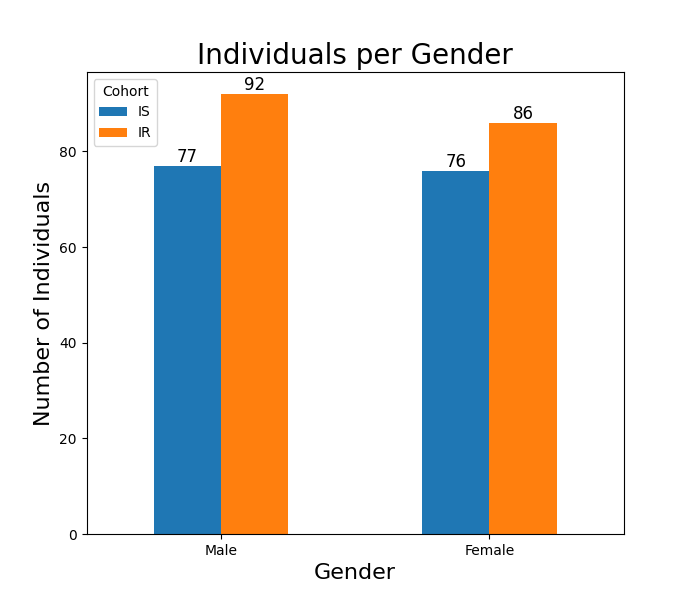
\includegraphics[width=\linewidth]{../plots/t2d/Gender_bar_chart.png}
\end{minipage}%
\begin{minipage}{0.66\linewidth}
   \centering
   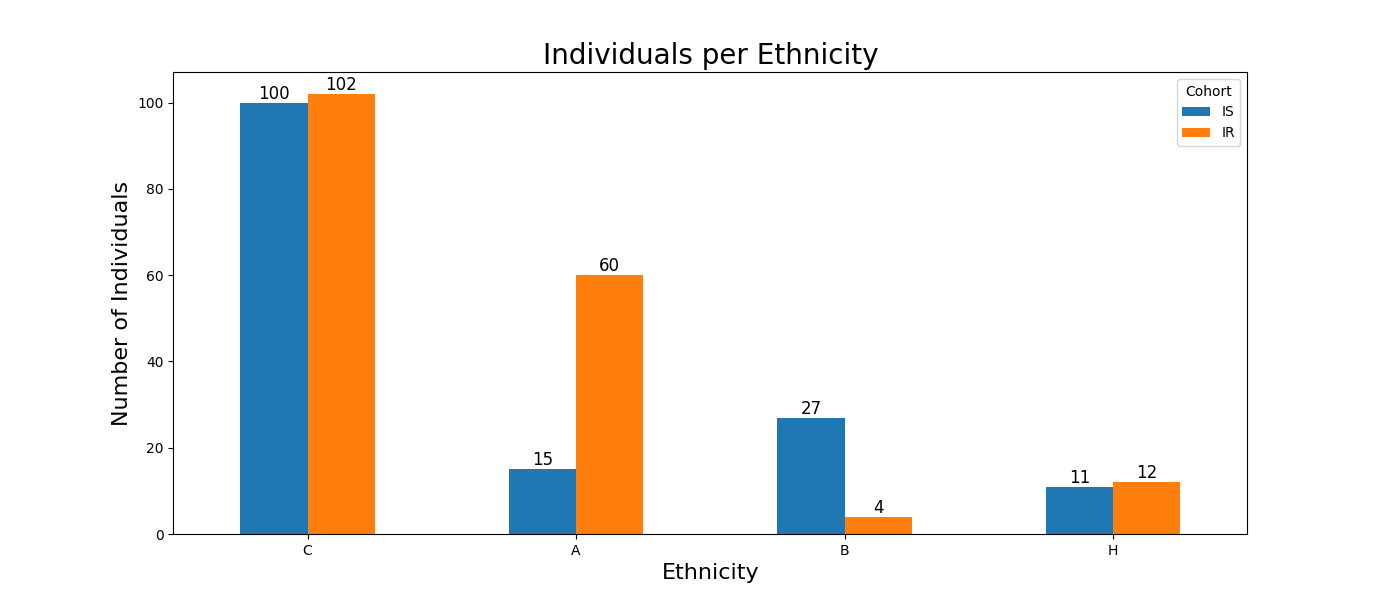
\includegraphics[width=\linewidth]{../plots/t2d/Ethnicity_bar_chart.png}
\end{minipage}
\caption{T2D Covariates Distribution}
\label{fig:t2dcovariates}
\end{figure}

\begin{figure}[h!]
\begin{minipage}{0.2\linewidth}
  \centering
  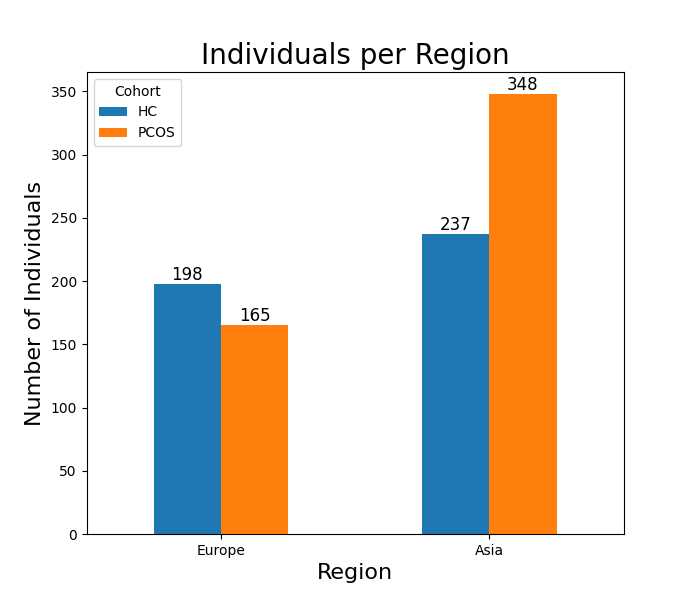
\includegraphics[width=\linewidth]{../plots/pcos/region_bar_chart.png}
\end{minipage}%
\begin{minipage}{0.8\linewidth}
   \centering
   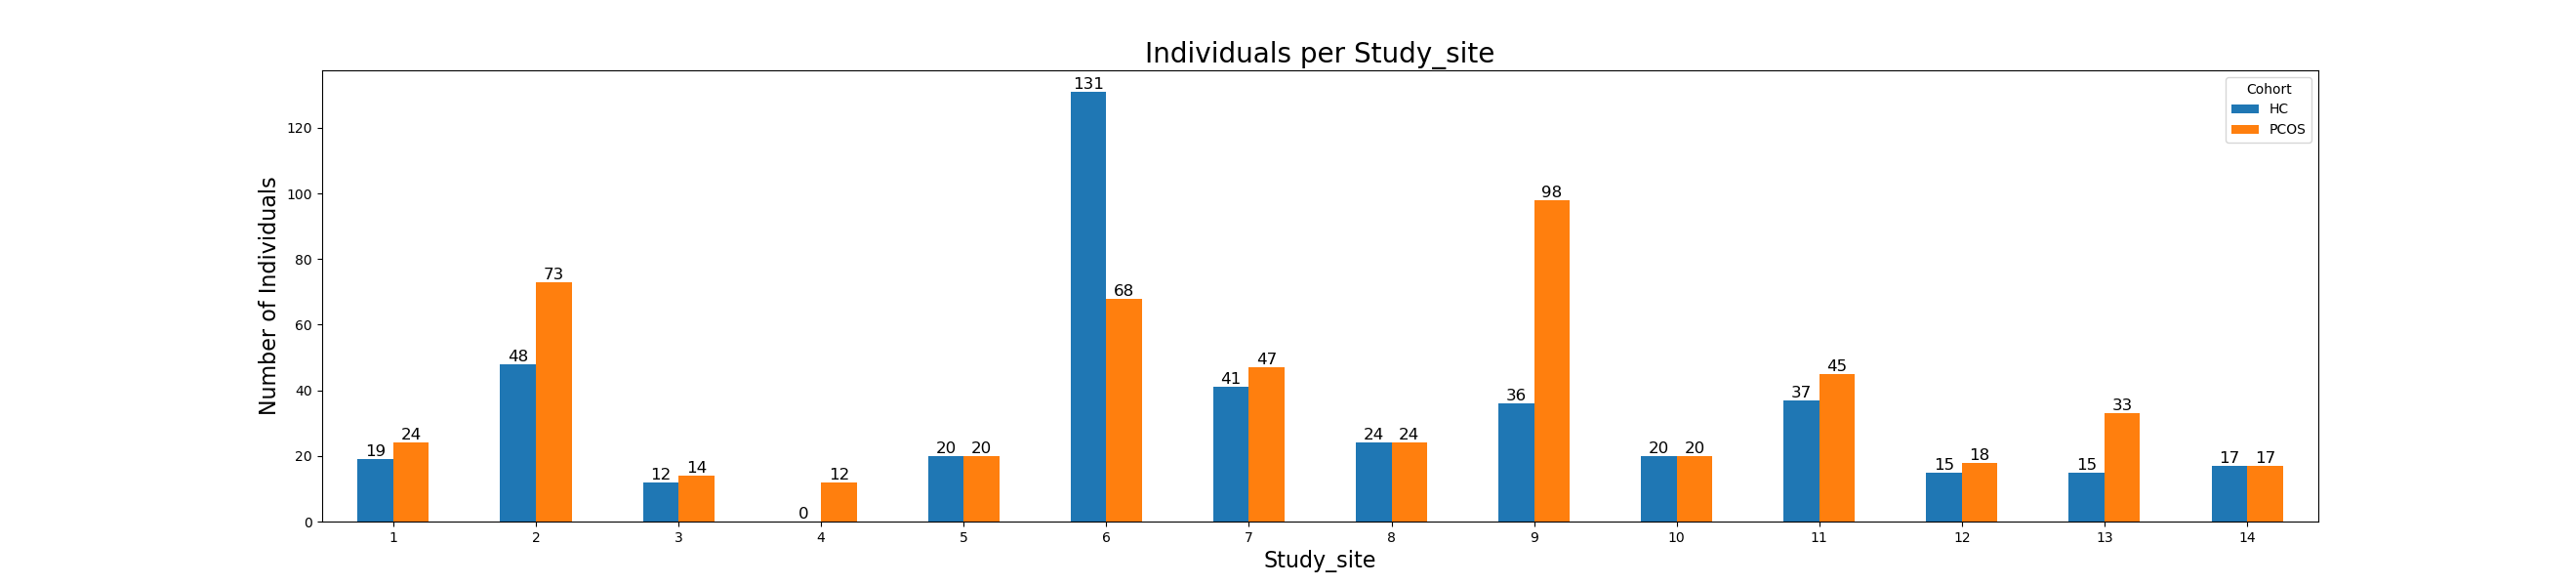
\includegraphics[width=\linewidth]{../plots/pcos/study_site_bar_chart.png}
\end{minipage}
\caption{PCOS Covariates Distribution}
\label{fig:pcoscovariates}
\end{figure}

\begin{figure}[h!]
   \centering
   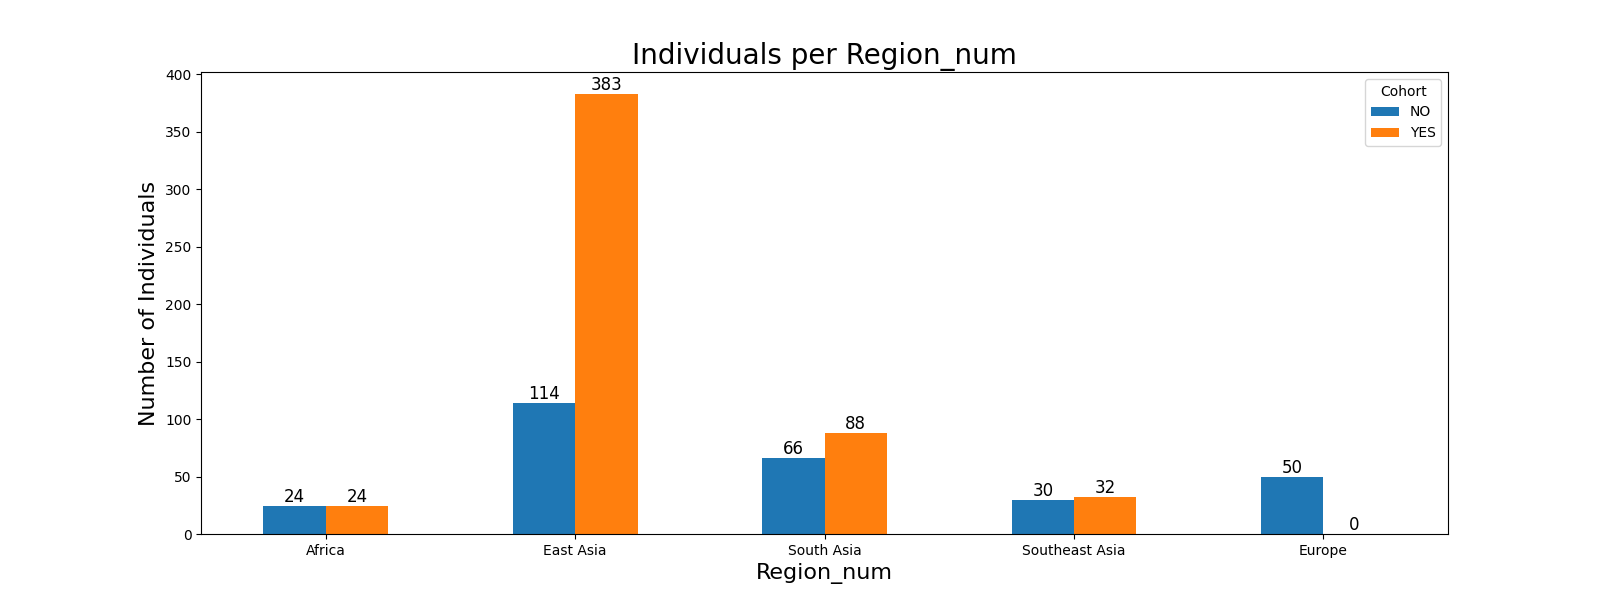
\includegraphics[width=\linewidth]{../plots/sam-t2d/region_num_bar_chart.png}
   \medskip
   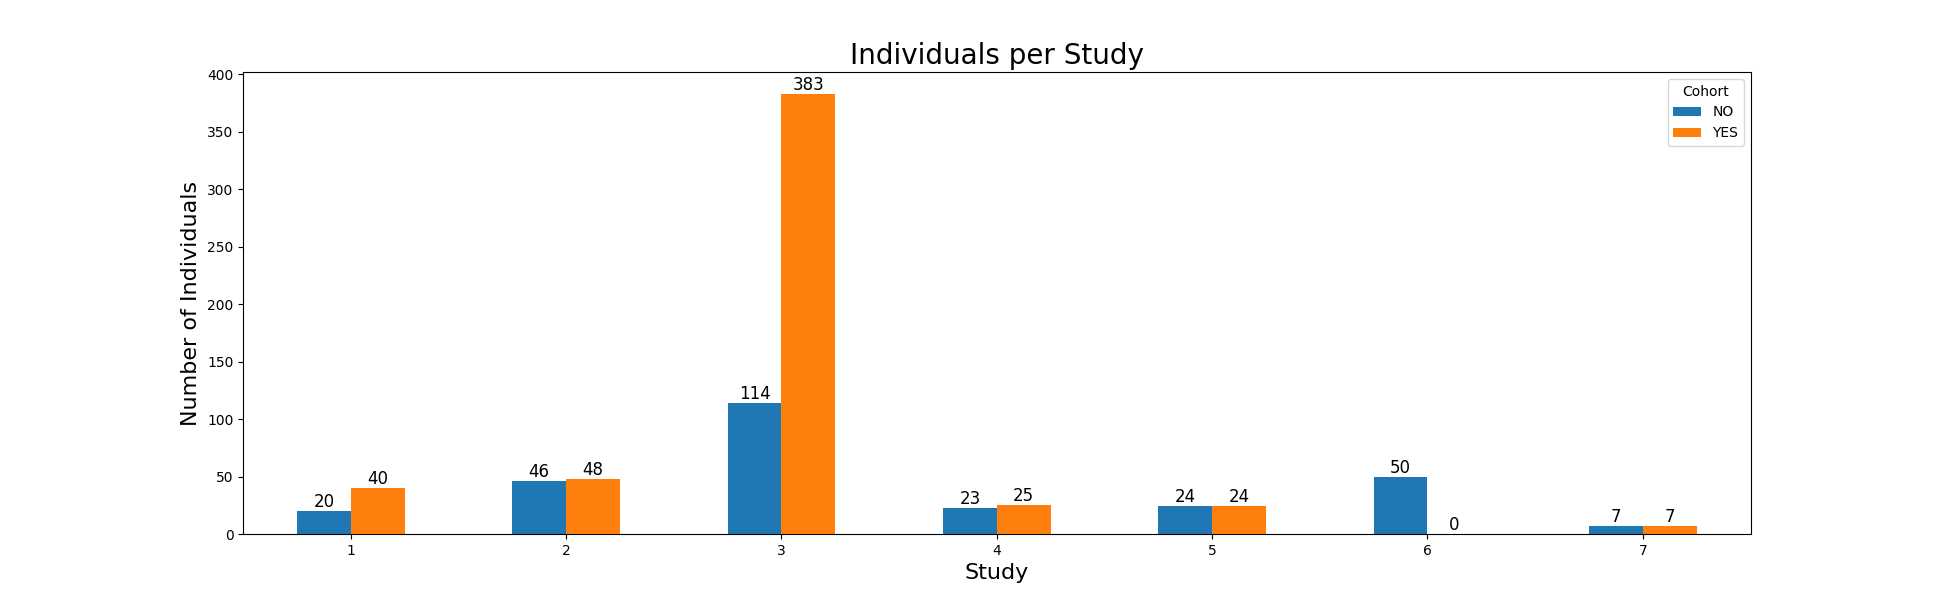
\includegraphics[width=\linewidth]{../plots/sam-t2d/study_bar_chart.png}
\caption{T2D Meta Analysis Covariates Distribution}
\label{fig:sam-t2dcovariates}
\end{figure}

We also check for linearity with scatter plots, and we check for normality with qqplots. Figure \ref{fig:t2dscatterplots} is a sample of scatter plots of pairs of microbes from the T2D dataset. Figure \ref{fig:t2dqqplots} is a sample of qqplots of microbes from the T2D dataset. We find that most microbes are non-linear and non-Gaussian, which means we need to be careful in selecting which independence tests to run and which models to fit. 

\begin{figure}[h!]
\begin{minipage}{0.47\linewidth}
  \centering
  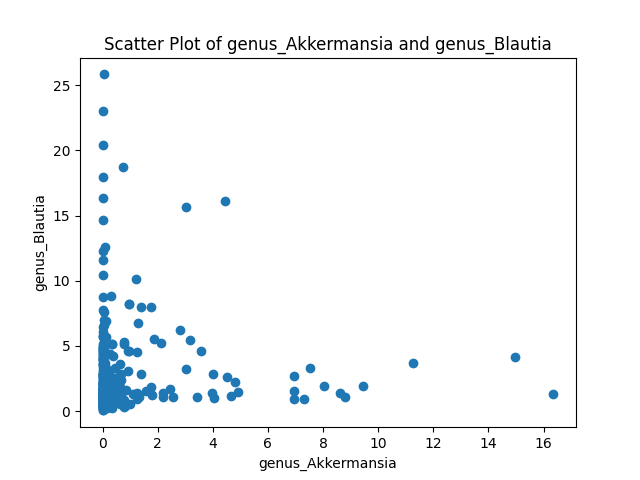
\includegraphics[width=\linewidth]{../plots/t2d/linearity/norm/genus_Akkermansia_vs_genus_Blautia.png}
\end{minipage}%
\begin{minipage}{0.47\linewidth}
   \centering
   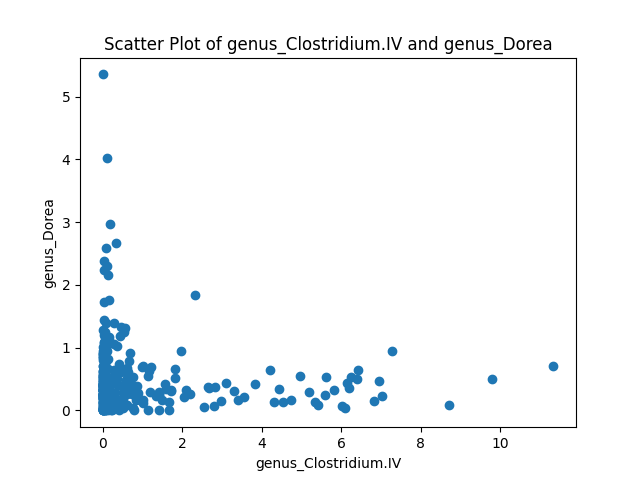
\includegraphics[width=\linewidth]{../plots/t2d/linearity/norm/genus_Clostridium.IV_vs_genus_Dorea.png}
\end{minipage}
\caption{T2D Scatter Plots for \textit{Akkermansia} vs. \textit{Blautia} and \textit{Clostridium IV} vs. \textit{Dorea}}
\label{fig:t2dscatterplots}
\end{figure}

\begin{figure}[h!]
\begin{minipage}{0.47\linewidth}
  \centering
  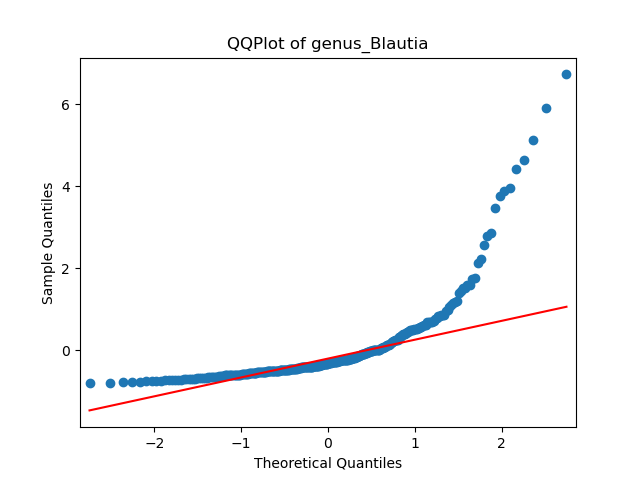
\includegraphics[width=\linewidth]{../plots/t2d/normality/norm/genus_Blautia.png}
\end{minipage}%
\begin{minipage}{0.47\linewidth}
   \centering
   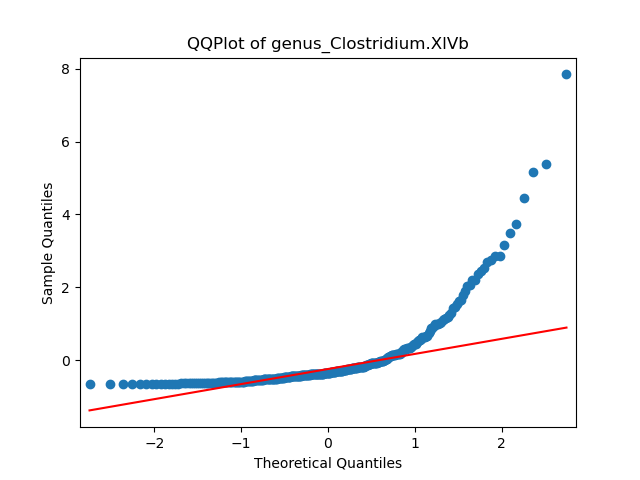
\includegraphics[width=\linewidth]{../plots/t2d/normality/norm/genus_Clostridium.XlVb.png}
\end{minipage}
\caption{T2D QQ Plots for \textit{Blautia} and \textit{Clostridium XIVb}}
\label{fig:t2dqqplots}
\end{figure}

\subsection{Microbe-Microbe Interaction Network}

To explore microbial interactions, we built microbe-microbe networks using SparCC and graphical lasso for feature selection. We then applied the PC algorithm with a max depth of 2 to infer causal relationships within these microbial networks. The following figures correspond to microbe-microbe networks where graphical lasso was applied as the feature selection method. The SparCC versions can be found in the Appendix.

\begin{figure}[h!]
  \centering
  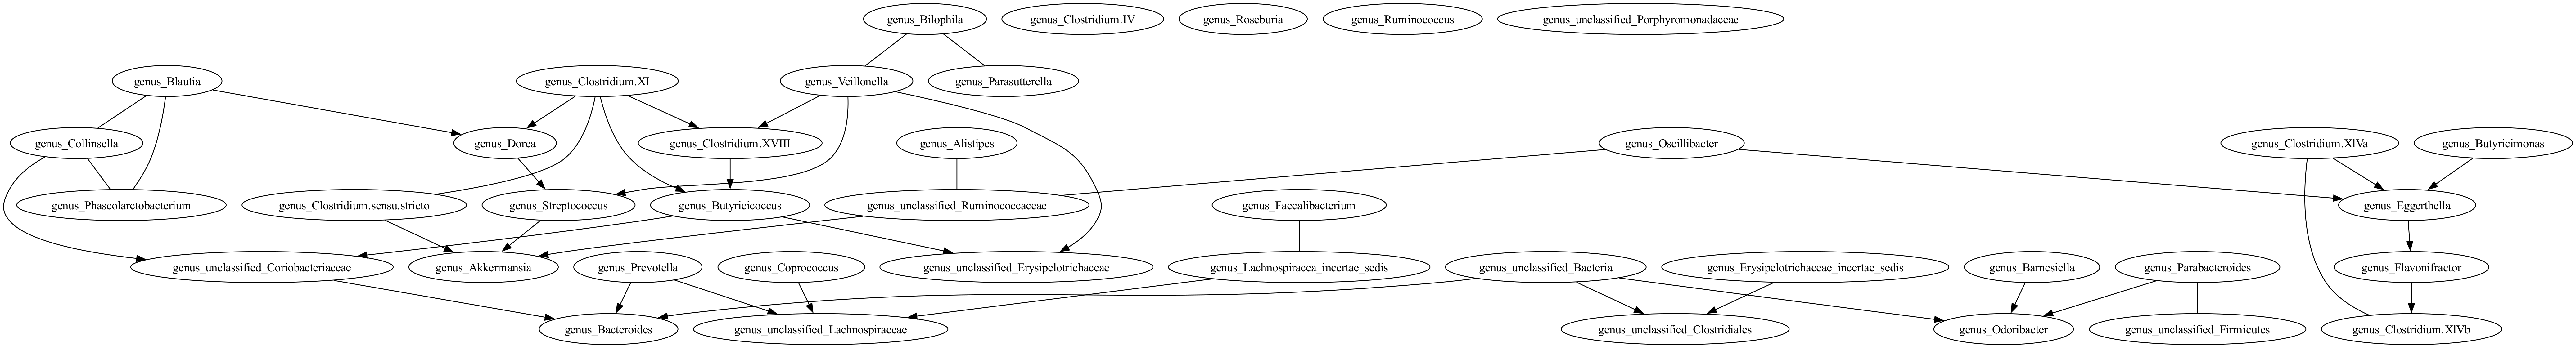
\includegraphics[width=\linewidth]{../graphs/t2d/glasso_IS_norm.png}
  \caption{T2D Microbe-Microbe Network for IS after Graphical Lasso}
  \label{fig:t2dglassoISnorm}
\end{figure}

\begin{figure}[h!]
  \centering
  
\includegraphics[width=\linewidth]{../graphs/t2d/glasso_IR_norm.png}
  \caption{T2D Microbe-Microbe Network for IR after Graphical Lasso}
  \label{fig:t2dglassoIRnorm}
\end{figure}

\begin{figure}[h!]
  \centering
  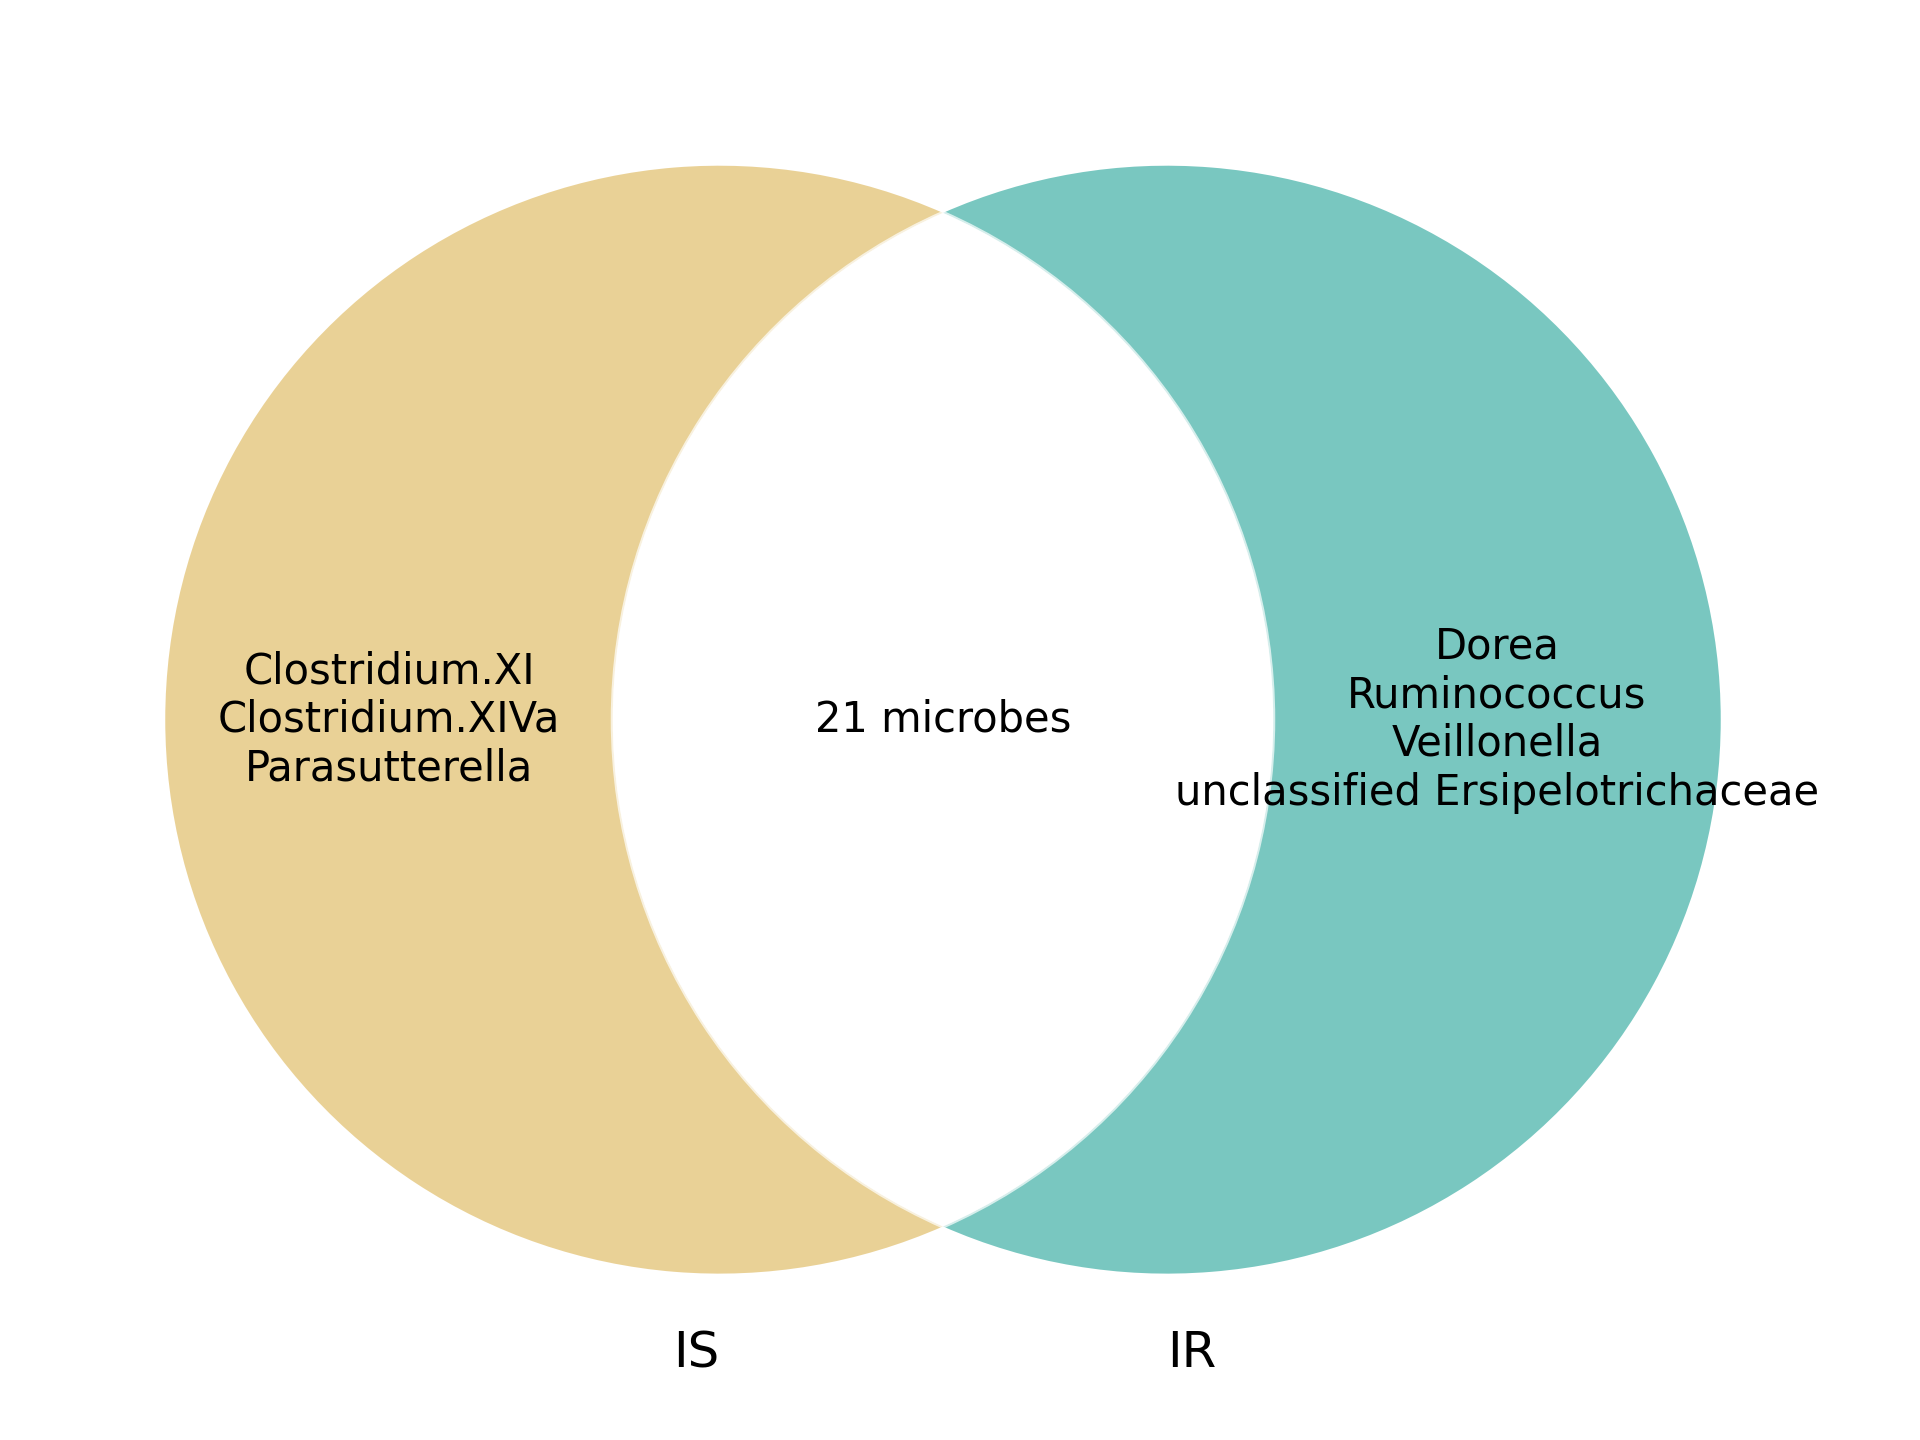
\includegraphics[width=0.8\linewidth]{../poster/t2d_microbe_microbe_venn.png}
  \caption{T2D Microbe-Microbe Network Venn Diagram}
  \label{fig:t2dglassovenn}
\end{figure}

For T2D, the two networks (Figures \ref{fig:t2dglassoISnorm} and \ref{fig:t2dglassoIRnorm}) found that both IR and IS cohorts share 21 microbes (Figure \ref{fig:t2dglassovenn}). The IS cohort has three additional genera: \textit{Clostridium XI, Clostridium XIVa}, and \textit{Parasutterella}. The IR cohort has four additional genera: \textit{Dorea, Ruminococcus, Veillonella}, and \textit{unclassified Ersipelotrichaceae}.

\begin{figure}[h!]
  \centering
  \includegraphics[width=\linewidth]{../graphs/pcos/glasso_HC_norm.png}
  \caption{PCOS Microbe-Microbe Network for HC after graphical lasso}
  \label{fig:pcosglassoHCnorm}
\end{figure}

\begin{figure}[h!]
  \centering
  \includegraphics[width=\linewidth]{../graphs/pcos/glasso_PCOS_norm.png}
  \caption{PCOS Microbe-Microbe Network for PCOS after graphical lasso}
  \label{fig:pcosglassoPCOSnorm}
\end{figure}

\begin{figure}[h!]
  \centering
  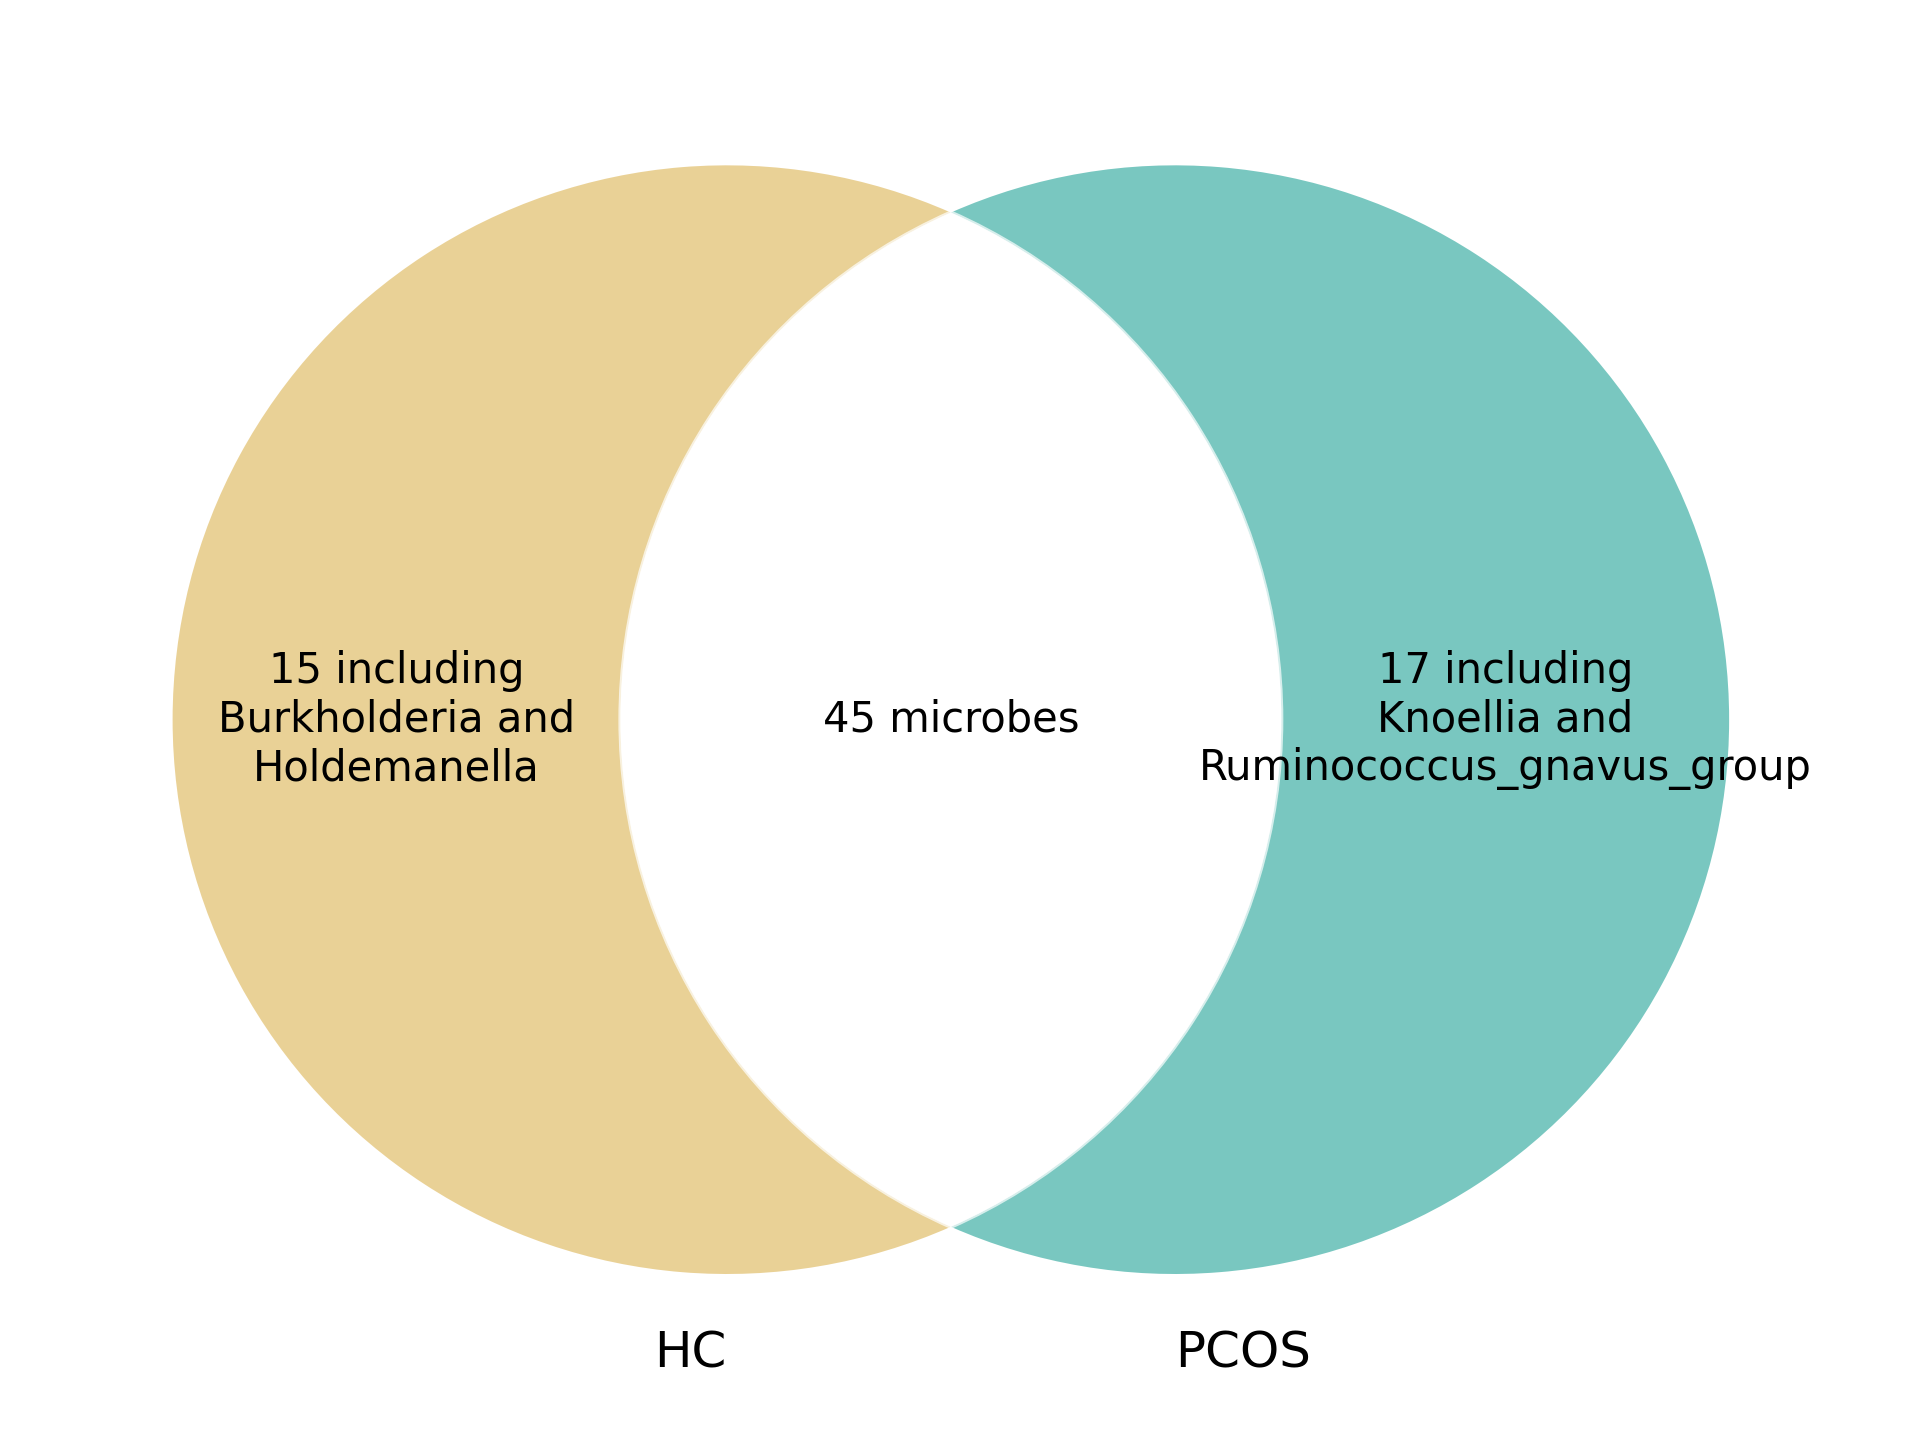
\includegraphics[width=0.8\linewidth]{../poster/pcos_microbe_microbe_venn.png}
  \caption{PCOS Microbe-Microbe Network Venn Diagram}
  \label{fig:pcosglassovenn}
\end{figure}

For PCOS, the two networks (Figures \ref{fig:pcosglassoHCnorm} and \ref{fig:pcosglassoPCOSnorm}) found that both HC and PCOS cohorts share 45 microbes (Figure \ref{fig:pcosglassovenn}). The HC cohort has 15 additional genera, which include \textit{Burkholderia} and \textit{Holdemanella}. The PCOS cohort has 17 additional genera, which include \textit{Knoellia} and \textit{Ruminococcus gnavus} group. 

For the T2D-meta analysis data, the two networks found that both non-T2D and T2D cohorts share 27 microbes. The non-T2D cohort has 10 additional genera including \textit{Sutterella} and \textit{Succinivibrio}. The T2D cohort has 13 additional genera including \textit{Lactobacillus} and \textit{Veillonella}. Due to the length of the taxa names and the width of the graph, the figures for T2D meta analysis can be found on our Github repo in higher resolution. 

\subsection{Microbe-Disease Interaction Network}

For the microbe-disease interaction networks, we used logistic lasso regression for feature selection and applied the CD-NOD algorithm with the non-microbe covariates as the heterogeneity index variables. For T2D, these are “Gender” and “Ethnicity”; for PCOS, these are “study/site” and “region”. We generated one causal graph for T2D and one for PCOS and identified the main microbial genera directly linked to the disease status nodes. For T2D, there were five genera: \textit{Butyricimonas, Clostridium XIVb, Odoribacter, unclassified Bacteria}, and \textit{unclassified Firmicutes}. For PCOS, there were nine genera: \textit{Alistipes, Blautia, Burkholderia, Desulfovibrio, Holdemanella, Knoellia, Prevotellaceae NK3B31 group, Ruminococcus}, and \textit{Ruminococcus gnavus group}. For the T2D meta analysis, there was one covariate (region), and there were eight genera directly linked to T2D: \textit{Alistipes\_A\_871400, Aphodomorpha, CAG-267, Collinsella, Faecalibacterium, Prevotella, Pseudobutyrivibrio,} and \textit{unclassified Monoglobaceae}. Due to the length of the taxa names and the width of the graph, the figures for T2D meta analysis can be found on our Github repo in higher resolution. 

\begin{figure}[h!]
  \centering
  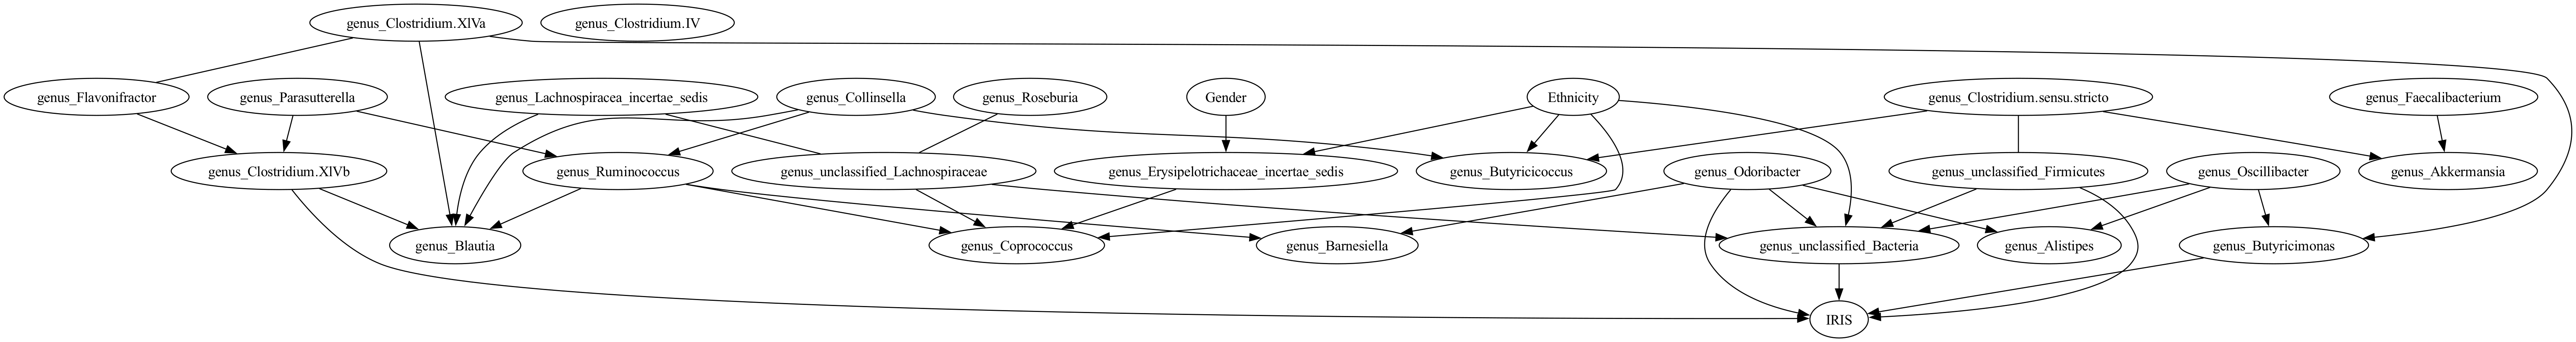
\includegraphics[width=\linewidth]{../graphs/t2d/cdnod_norm.png}
  \caption{T2D Microbe-Disease Network}
  \label{fig:t2dcdnod}
\end{figure}

\begin{figure}[h!]
  \centering
  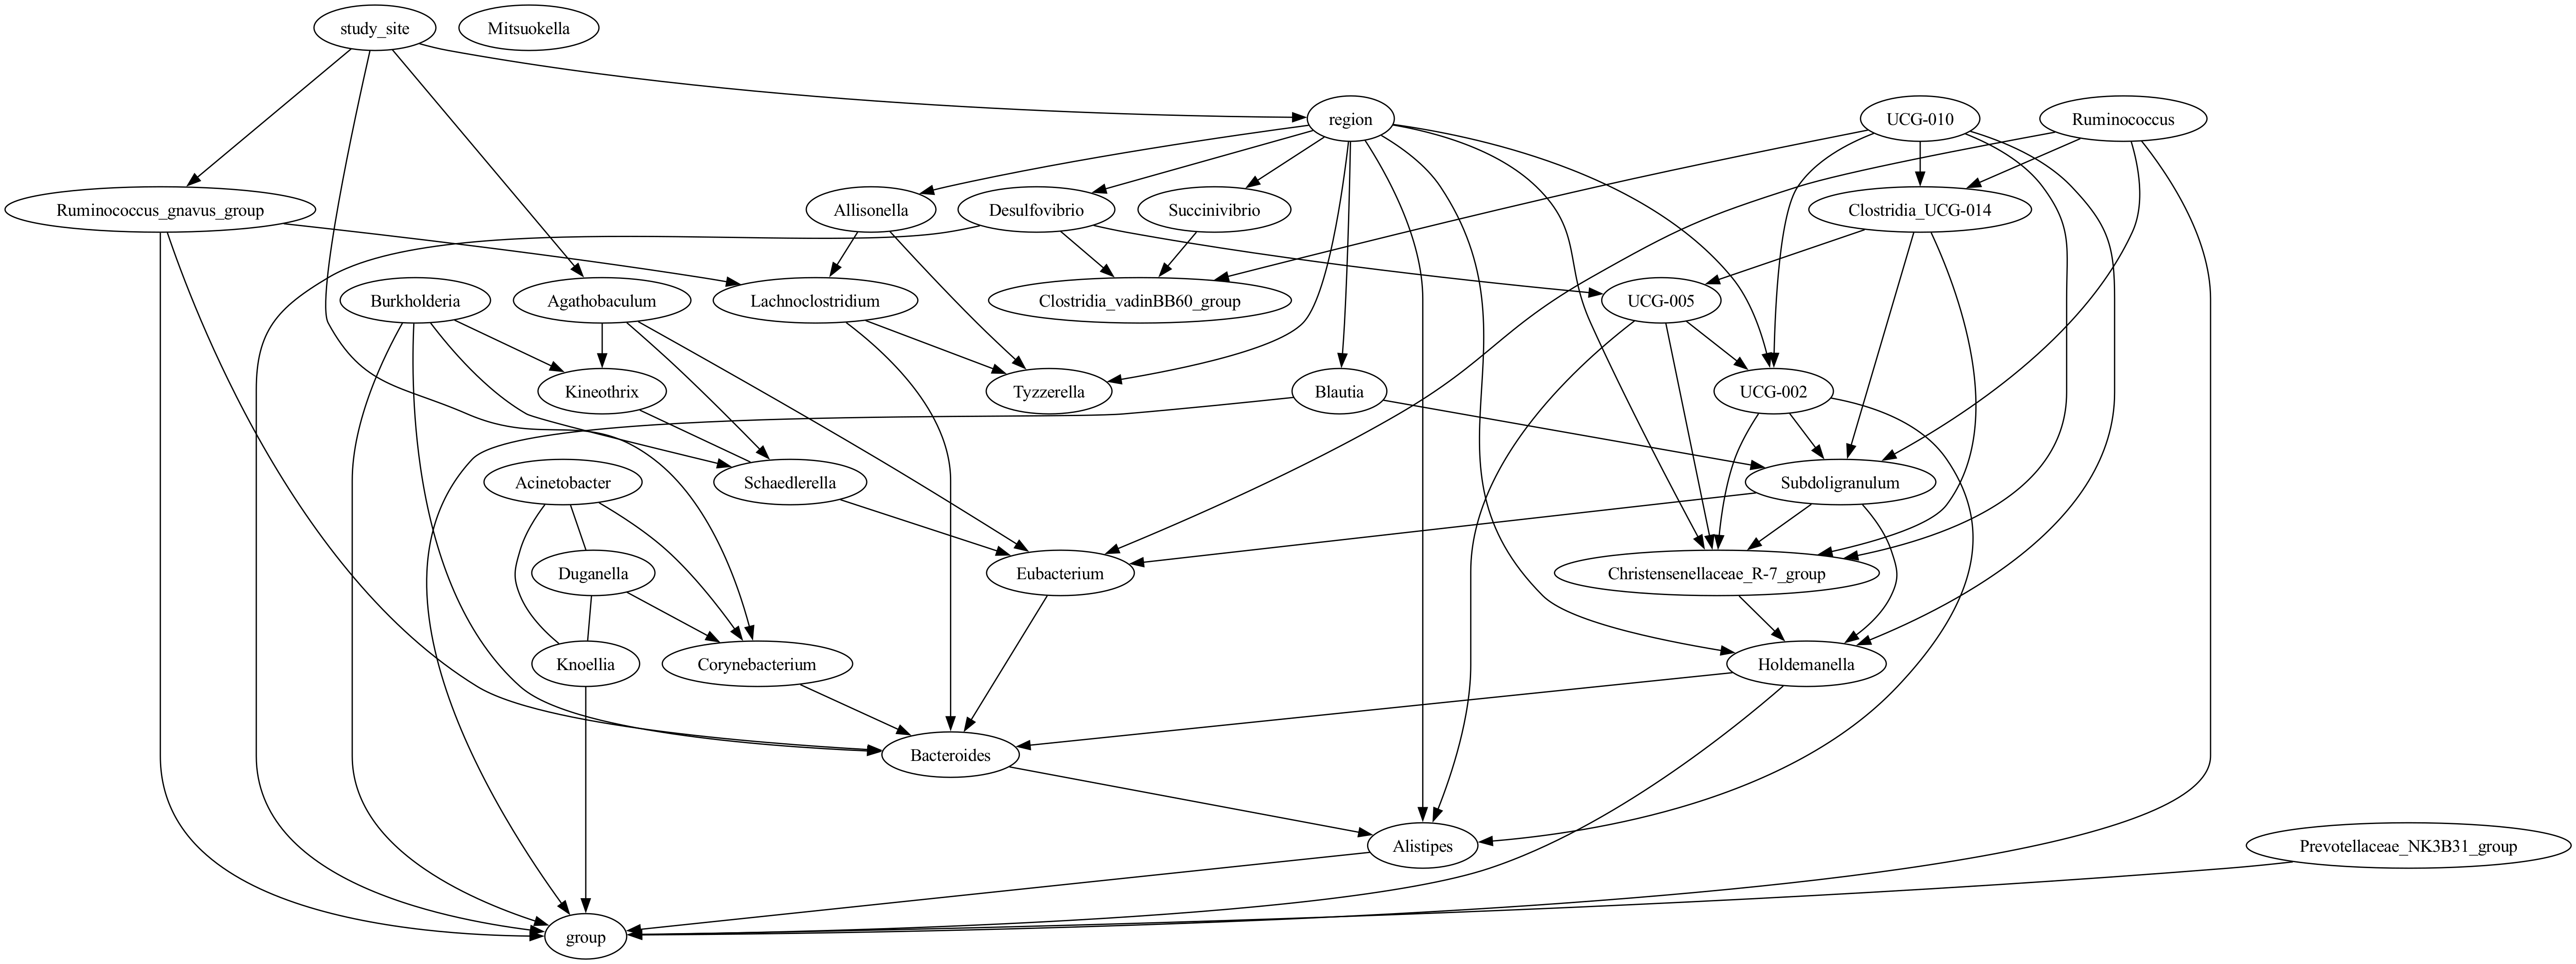
\includegraphics[width=\linewidth]{../graphs/pcos/cdnod_norm.png}
  \caption{PCOS Microbe-Disease Network}
  \label{fig:pcoscdnod}
\end{figure}

\subsection{Causal Inference and BIRDMAn}

To strengthen our causal interpretations, we applied do-calculus to estimate the effect of each genera while accounting for confounders. Model 1 used logistic regression to estimate the effects of the directly linked microbes to disease status, and essentially considers the directly linked microbes as a community of microbes. For example, the model for the T2D graph is: \begin{align*}\text{logit(IRIS)} = &\beta_0 + \beta_1 \textit{Butyricimonas} + \beta_2 \textit{Clostridium XIVb}\\ &+ \beta_3 \textit{Odoribacter} + \beta_4 \textit{unclassified Bacteria} + \beta_5 \textit{unclassified Firmicutes}\end{align*}
where we are interested in $\beta_1, \dots, \beta_5$ for the effect of \textit{Butyricimonas}, …, \textit{unclassified Firmicutes}, respectively.

Model 2 tries a different approach by estimating the marginal effects of each of the directly linked microbes to disease status by incorporating the microbe’s neighbors and mediators to adjust for potential indirect effects. For example, one of the models for the T2D graph are: \[\textit{logit(IRIS)} = \beta_0 + \beta_1 \textit{Butyricimonas} + \beta_2 \textit{Clostridium XIVa} + \beta_3 \textit{Oscillibacter}\]
where we are interested in $\beta_1$ for the effect of \textit{Butyricimonas}. This model only needs to account for the neighbors of \textit{Butyricimonas} (\textit{Clostridium XIVa} and \textit{Oscillibacter}) to obtain the effect. 

On the other hand, \textit{Odoribacter} and \textit{unclassified Firmicutes} are mediated by \textit{unclassified Bacteria}. We have to use a different method to estimate the total direct effect of \textit{Odoribacter} and \textit{unclassified Firmicutes} by estimating the direct effect of \textit{Odoribacter} and \textit{unclassified Firmicutes}, and adding their indirect effects through the mediator. For example, the models for \textit{Odoribacter} are:
\[\textit{unclassified Bacteria} = \theta_0 + \theta_1 \textit{Odoribacter}\]
\[\textit{logit(IRIS)} = \beta_0 + \beta_1 \textit{Odoribacter} + \beta_2 \textit{unclassified Bacteria} + \beta_3 \textit{Alistipes} + \beta_4 \textit{Barnesiella}\]
where we compute the total direct effect as $\beta_1 + \theta_1\beta_2$. 

Additionally, we utilized Bayesian inference through BIRDMAn, using a negative binomial model to conduct a more traditional differential analysis that is commonly used in gut microbiome studies. BIRDMAn tells us the mean CLR of each microbe’s abundance and ranks them based on their mean CLRs. We are interested in comparing the directions of the values of these three models, to ensure that they all agree on whether a microbe is harmful or beneficial to odds or risk of disease. Their magnitudes may be different because they are all different models, and we do not imply that any of the models are better than the others, or that one value should be trusted more than the others. We also check with the current literature to see if the biological mechanisms of these microbes and associated metabolites and relation to disease agree. 

\begin{table}
        
        \centering
        \begin{tabular}{l r r r c}
          \toprule
          \textbf{Genus} & \textbf{Model 1} & \textbf{Model 2} & \textbf{BIRDMAn} & \textbf{Literature Agreement} \\
          \midrule
          \textit{Butyricimonas} & -2.0070* & -2.26645* & -5.19385* & Yes \\
          \textit{Clostridium XIVb} & 1.54212* & 1.80822* & 2.15788* & Inconclusive \\
          \textit{Odoribacter} & -1.46989* & -3.055047* & -2.43796* & Yes \\
          \textit{unclassified Bacteria} & -0.12991* & -0.12284* & 0.12409 & N/A \\
          \textit{unclassified Firmicutes} & -0.69477* & -0.933718* & -1.47437* & N/A \\
          \bottomrule
        \end{tabular}
        \caption{Log-Odds Ratios for Models 1 \& 2, and Mean CLR from BIRDMAn for T2D.}
        \label{table:t2dresults}
      \end{table}
      
      \begin{table}
        \centering
        \begin{tabular}{l r r r c}
          \toprule
          \textbf{Genus} & \textbf{Model 1} & \textbf{Model 2} & \textbf{BIRDMAn} & \textbf{Literature Agreement} \\
          \midrule
          \textit{Alistipes} & 0.13272* & 0.15346* & 1.28613* & Inconclusive \\
          \textit{Blautia} & 0.07461* & 0.07008* & 0.82554* & No \\
          \textit{Burkholderia} & -7.60599 & -0.48578 & -10.95696* & Inconclusive \\
          \textit{Desulfovibrio} & -0.79283* & -1.14492* & -0.17153 & No \\
          \textit{Holdemanella} & -0.22801* & -0.17267* & -0.13299 & Yes \\
          \textit{Knoellia} & 592.26751 & 1.40864 & 5.57650* & Inconclusive \\
          \textit{Prevotellaceae NK3B31 group} & -0.42407 & -0.47231* & -1.76743* & Inconclusive \\
          \textit{Ruminococcus} & -0.14137* & -0.13490* & -0.12796 & Inconclusive \\
          \textit{Ruminococcus gnavus group} & 0.24152* & 0.18259* & 2.01842 & Yes \\
          \bottomrule
        \end{tabular}
        \caption{Log-Odds Ratios for Models 1 \& 2, and Mean CLR from BIRDMAn for PCOS.}
        \label{table:pcosresults}
      \end{table}
      
\begin{table}
        \centering
        \begin{tabular}{l r r r c}
          \toprule
          \textbf{Genus} & \textbf{Model 1} & \textbf{Model 2} & \textbf{BIRDMAn} & \textbf{Literature Agreement} \\
          \midrule
          \textit{Alistipes\_A\_871400} & -0.72608* & -0.87070* & -1.38028 & Inconclusive \\
          \textit{Aphodomorpha} & -1.23747* & -2.36658* & -1.54138* & Inconclusive \\
          \textit{CAG-267} & -19.68728 & -13.81186 & N/A & Inconclusive \\
          \textit{Collinsella} & 0.10462* & 0.08761* & 1.14355* & Yes \\
          \textit{Faecalibacterium} & -0.10471* & -0.07721* & -0.09936 & Yes \\
          \textit{Prevotella} & -0.02734* & -0.01884* & -0.25227* & Yes \\
          \textit{Pseudobutyrivibrio} & 1.80315* & 1.76850* & 2.80971* & Inconclusive \\
          \textit{unclassified Monoglobaceae} & -9.38222* & -8.98766* & -4.07403* & N/A \\
          \bottomrule
        \end{tabular}
        \caption{Log-Odds Ratios for Models 1 \& 2, and Mean CLR from BIRDMAn for T2D Meta-Analysis.}
        \label{table:sam-t2dresults}
      \end{table}


Table \ref{table:t2dresults} shows the coefficients obtained in Model 1 and Model 2 for the five microbes, as well as their BIRDMAn mean CLR values. Significant values ($\alpha < 0.05$) are denoted by *. The most important part of the results is the sign of the values. For example, \textit{Butyricimonas, Odoribacter, unclassified Bacteria}, and \textit{unclassified Firmicutes} have negative values, which means that they are protective towards T2D. We consult with the literature on the biological mechanisms of these microbes that are available and currently known to check that our results make sense. Table \ref{table:pcosresults} shows the same results for the PCOS dataset, and Table \ref{table:sam-t2dresults} shows the same results for the T2D meta-analysis. 

\subsection{VAE Model}

xxx

\section{Discussion}

Our study shows that specific gut microbes may play a direct role in metabolic diseases like T2D and PCOS. We found significant microbes that affect T2D and PCOS, and find that they agree between the two do-calculus results and BIRDMAn differential analysis. Now, we explain why these make sense in terms of their biological mechanisms in relation to T2D and PCOS. We also find different results for the T2D dataset from HMP2 vs the meta analysis because the study participants are from different regions. 

In T2D, the first significant microbe in our table is \textit{Butycrimonas}. Our causal inference results suggest that it plays a protective role, with a $e^{-2.26645} = 0.10368 =$ 90\% decrease in the odds of insulin resistance for a one percent increase in its abundance whilst its neighbors remain constant, which aligns with current literature. \textit{Butyricimonas} is generally considered beneficial for metabolic health. It is a butyrate-producing bacterial genus, and butyrate is a short-chain fatty acid (SCFA) that has multiple positive effects on metabolism \citep{lee2022butyricimonas}. Additionally, \textit{Odoribacter}, also known for its butyrate-producing properties \citep{albataineh2023odoribacter}, was associated with an $e^{-3.05501} = 0.04712 =$ 95\% decrease in the odds of insulin resistance for a one percent increase in its abundance whilst its neighbors remain constant, reinforcing its potential protective effect.

For PCOS, our results highlight \textit{Blautia} as a harmful microbe (its effect is negative). Unfortunately, this disagrees with literature: multiple studies have shown a decrease in \textit{Blautia} levels in individuals with PCOS, as well as in those with diabetes and obesity. This aligns with our findings and reinforces \textit{Blautia}’s role in metabolic health. The genus is also associated with lipid and glucose metabolism, and its ability to produce short-chain fatty acids (SCFAs) suggests a protective function against metabolic dysfunction \citep{li2023blautia}. Given that SCFAs influence insulin sensitivity and inflammation, \textit{Blautia} may be a key player in gut microbiome-driven metabolic regulation. In contrast, \textit{Desulfovibrio} appears to have a protective effect in PCOS from our results. This result also disagrees with literature: this genus belongs to a group of sulfate-reducing bacteria (SRB) that have been linked to chronic inflammation. Overgrowth of \textit{Desulfovibrio} has been observed in conditions like inflammatory bowel disease (IBD) and periodontitis, both of which involve gut dysbiosis and systemic inflammation \citep{singh2023desulfovibrio}. Another significant microbe is \textit{Holdemanella}, which we identified as beneficial. \textit{Holdemanella} has been shown to produce metabolites with strong anti-inflammatory properties. Some studies even suggest it plays a role in regulating GLP-1, a hormone crucial for blood sugar control and metabolic function \citep{romani2021holdemanella}. Additionally, our microbe-microbe network analysis revealed that \textit{Holdemanella} is linked to \textit{Collinsella} and \textit{Lactobacillus}, two genera with known roles in gut health and metabolism. This suggests that \textit{Holdemanella}’s effects may extend beyond its direct metabolic contributions, potentially influencing a broader microbial network that supports host health. On the other hand, the \textit{Ruminococcus gnavus group} was identified as harmful. This genus has been consistently associated with gut dysbiosis and inflammation in conditions such as IBD \citep{crost2023rgnavus}. Given the emerging evidence that PCOS and IBD share some common inflammatory pathways, the presence of \textit{Ruminococcus gnavus} may contribute to the chronic inflammation observed in PCOS. 

The T2D meta analysis results (Table \ref{table:sam-t2dresults}) show that \textit{Collinsella, Faecalibacterium}, and \textit{Prevotella} had significant effects and agreement with literature. In particular, \textit{Collinsella} has been found to be positively correlated with producing insulin, and also has been found to be a result of low dietary fiber \citep{gomez2018collinsella}, in contrast with intaking high dietary fiber which produces more SCFA-producing bacteria such as \textit{Prevotella} and is overall beneficial to metabolism \citep{abdelsalam2023prevotella}. \textit{Faecalibacterium} has been found in many studies to be negatively associated with T2D, and is also a popular probiotic for colitis which is an inflammatory disease of the colon \citep{gurung2020faecalibacterium}. 

For the other microbes in our results, such as \textit{Clostridium XIVb, Alistipes, Burkholderia}, and more, the evidence remains inconclusive. Studies on these genera report mixed findings, with some species and strains showing beneficial effects and others being harmful. Because our analysis operates at the genus level, we cannot distinguish between species with contrasting effects, making it difficult to classify them as definitively beneficial or harmful. This is a limitation of our study and the taxonomy classification step in general because strain-level differences within the same genus may play an important role in metabolic health. Additionally, the unclassified genera cannot be searched in literature because they may contain all kinds of genera and are just a category for the microbes that could not be classified. 

\subsection{Limitations}

There remain a few limitation to our project that encompass some of the limitations commonly found in gut microbiome research. First, it is difficult to convince researchers that our results are “causal” because the gut microbiome is constantly changing. It can vary throughout the year, seasons, and even during the day as people consume food or alcohol, take medications, and encounter stressful situations. Thus, gut microbiome longitudinal studies are often the best study design to assess causality. It is still difficult to collect many samples of longitudinal data that are consistent and account for all confounding variables, but we believe our pipeline can still be applied to these data when it is available. There may also be better causal discovery and causal inference methods that account for such longitudinal structures. 

The lack of accounting for confounding is also a limitation as it pertains to causal discovery, where we assume no hidden confounders for algorithms like PC and CD-NOD. However, we know that there are many potential confounding variables to the gut microbiome, and our datasets did not include variables for them. Thus, the results may change drastically depending on how well confounding variables are accounted for in the data. 

There is one particular confounding variable that can be problematic in the case of meta analyses: study id. In gut microbiome data, samples that come from the same study are often very related because the study uses the same sequencing and classification methods to produce the OTU table. The classification methods are also not 100\% accurate; common classifiers may have 80-90\% accuracy, meaning there is already some error in the data. The taxonomies that it produces also depend on the OTUs that are only present in those samples, so when combining the OTU tables of multiple studies, we will often see blocks, where an OTU has non-zero values only in particular studies. Additionally, people of different regions of the world will have different diets which can have a large impact on their gut microbiome compositions. Those living in similar regions will thus have similar gut microbiome compositions compared to two very different regions. 

Another gut microbiome-specific limitation is addressing the rarity of a certain microbe. A microbe may be considered rare in a dataset, i.e. it has a low abundance, due to two reasons: (1) the microbe is rare as a result of the artifact, or (2) the microbe is truly rare in the gut. The former issue is a result of the sequencing instrument only containing a fixed number of slots where gut microbe DNA can fit, so a microbe that appears rare may only be rare since it did not make it into one of the slots of the sequencing instrument. One way to address this issue is to perform a centered-log ratio transformation on each sample (the log of the proportion of the count over the geometric mean of the sample) to reduce the disparity between rare microbe values and abundant microbe values. However, this makes the interpretation of each feature relevant to all other features on the log scale and the results must be interpreted as such. 

Finally, in terms of causal discovery algorithms, we face issues of low statistical power when performing many conditional independence tests due to the high-dimensional nature of the data. It is also difficult to obtain large samples (anything over 1,000) in gut microbiome studies, and one way to address low statistical power from multiple testing is to apply a multiple testing correction, such as on the false discovery rate. However, there are currently no concrete multiple testing corrections for causal discovery algorithms, and the power and multiple testing problem remains to be a limitation.


\subsection{Improvements and Future Directions}

In addition to addressing the limitations described above, we hope our pipeline’s results can be verified with experiments and further research on the biological mechanisms of gut microbes, as is traditionally done to prove causality. We also hope that our pipeline can be applied to gut microbiome data on other diseases, and that it can be further improved in the choice of algorithms and methods with respect to the data characteristics, e.g. sparsity, compositionality, longitudinal/time series. 

As we use BIRDMAn as a benchmark tool for differential analysis methods, we can also benchmark our results with other differential analysis and network methods that exist and are popular in gut microbiome research today. We hope that further development in this area of microbiome analysis can also allow us to assess our pipeline on more sophisticated methods. 

\section{Conclusion}

xxx

%%%%%%%%%%%%%%%%%%%%%%%%%%%%%%%%%%%%%%%%%%%%%%%%%%%%%%%%
%%%% Reference / Bibliography
%%%%%%%%%%%%%%%%%%%%%%%%%%%%%%%%%%%%%%%%%%%%%%%%%%%%%%%%

\clearpage
\makereference

\bibliography{reference}
\bibliographystyle{style/dsc180bibstyle}
% \bibstyle{style/dsc180bibstyle}

%%%%%%%%%%%%%%%%%%%%%%%%%%%%%%%%%%%%%%%%%%%%%%%%%%%%%%%%
%%%% Appendix
%%%%%%%%%%%%%%%%%%%%%%%%%%%%%%%%%%%%%%%%%%%%%%%%%%%%%%%%

\clearpage
\makeappendix

Please see a copy of our \href{https://drive.google.com/file/d/1fEGpmoSULPbpG6bcopPBKdlyF6gG_Gv_/view?usp=sharing}{project proposal}. 

\subsection{T2D Meta-Analysis Metadata}

(Insert T2D Metadata)

\subsection{Algorithms}

\begin{algorithm}[H]
\caption{PC}
\label{alg:pc}
\DontPrintSemicolon
\LinesNumbered
\KwIn{Data, $\mathbf D$}
\KwOut{CPDAG, $G$}
$G \gets \text{the complete undirected graph over $\mathbf D$}$\;
$\textbf{Sepset}(A, B) = \textbf{Sepset}(B, A) \gets \emptyset \quad \text{(the d-separation set of $A$ and $B$ $\forall A, B \in G$)}$\;
\tcp{Causal skeleton discovery}
\For{$(A, B)$ adjacent pairs in $G$} {
    $n \gets 0$\;
    \While{$\exists$ a set $C$ in $G$ adjacent to $A$ or $B$ s.t. $|C| = n$}{
        \If{$A \ind B | C$} {
            $\text{remove the edge between $A$ and $B$}$\;
            $\text{record $C$ in \textbf{Sepset}$(A, B)$ and \textbf{Sepset}$(B, A)$}$\;
            \textbf{break}
        }
        $n \gets n + 1$\;
    }
}
\tcp{Find v-structures}
\For{$(A, B, C)$ triple in $G$ s.t. $A - B - C$}{
    \If{$B \notin \textbf{Sepset}(A, C)$}{
        $\text{orient the edges $A \to B \leftarrow C$}$\;
    }
}
\tcp{Orientation propagation via Meek rules}
\While{there are edges to orient} {
    \If{$A \to B$, and $B$ and $C$ are adjacent, and $A$ and $C$ are not adjacent, and there is no arrowhead at $B$} {
        $\text{orient the edge $B - C$ as $B \to C$}$\;
    }
    \If{$\exists$ a directed path from $A$ to $B$, and an edge between $A$ and $B$}{
        $\text{orient the edge $A - B$ as $A \to B$}$\;
    }
}
\end{algorithm}

\begin{algorithm}[H]
\caption{CD-NOD}
\label{alg:cdnod}
\DontPrintSemicolon
\LinesNumbered
\KwIn{Data, $\mathbf D$ which has variable set $\mathbf V$; surrogate $\mathbf C$}
\KwOut{CPDAG, $G$}
$G \gets \text{the complete undirected graph over $\mathbf V \cup \mathbf C$}$\;
\tcp{Detect changing causal modules}
$\textbf{Sepset}(V_i, C) \gets \emptyset \quad \text{(the d-separation set of $V_i$ and $C$ $\forall V_i \in \mathbf V$)}$\;
\For{$V_i$ in $\mathbf V$}{
    $n \gets 0$\;
    \While{$\exists$ a set $S = \{V_k | k \neq i\}$ in $G$}{
        \If{$V_i \ind C | S$}{
            $\text{remove the edge between $V_i$ and $C$}$\;
            $\text{record $S$ in \textbf{Sepset}$(V_i, C)$}$\;
            \textbf{break}
        }
        $n \gets n + 1$\;
    }
}
\tcp{Causal skeleton discovery}
$\textbf{Sepset}(A, B) = \textbf{Sepset}(B, A) \gets \emptyset \quad \text{(the d-separation set of $A$ and $B$ $\forall A, B \in G$)}$\;
\For{$(A, B)$ adjacent pairs in $G$} {
    $n \gets 0$\;
    \While{$\exists$ a set $C$ in $G$ adjacent to $A$ or $B$ s.t. $|C| = n$}{
        \If{$A \ind B | C \cup \mathbf C$} {
            $\text{remove the edge between $A$ and $B$}$\;
            $\text{record $C$ in \textbf{Sepset}$(A, B)$ and \textbf{Sepset}$(B, A)$}$\;
            \textbf{break}
        }
        $n \gets n + 1$\;
    }
}
\tcp{Find v-structures}
\For{$(A, B, C)$ triple in $G$ s.t. $A - B - C$}{
    \If{$B \notin \textbf{Sepset}(A, C)$}{
        $\text{orient the edges $A \to B \leftarrow C$}$\;
    }
}
\end{algorithm}

\begin{algorithm}[H]
\DontPrintSemicolon
\LinesNumbered
\setcounter{AlgoLine}{30}
\tcp{Orientation propagation via Meek rules}
\While{there are edges to orient} {
    \If{$A \to B$, and $B$ and $C$ are adjacent, and $A$ and $C$ are not adjacent, and there is no arrowhead at $B$} {
        $\text{orient the edge $B - C$ as $B \to C$}$\;
    }
    \If{$\exists$ a directed path from $A$ to $B$, and an edge between $A$ and $B$}{
        $\text{orient the edge $A - B$ as $A \to B$}$\;
    }
}
\end{algorithm}

\subsection{SparCC Microbe-Microbe Interaction Networks}

\begin{figure}[h!]
  \centering
  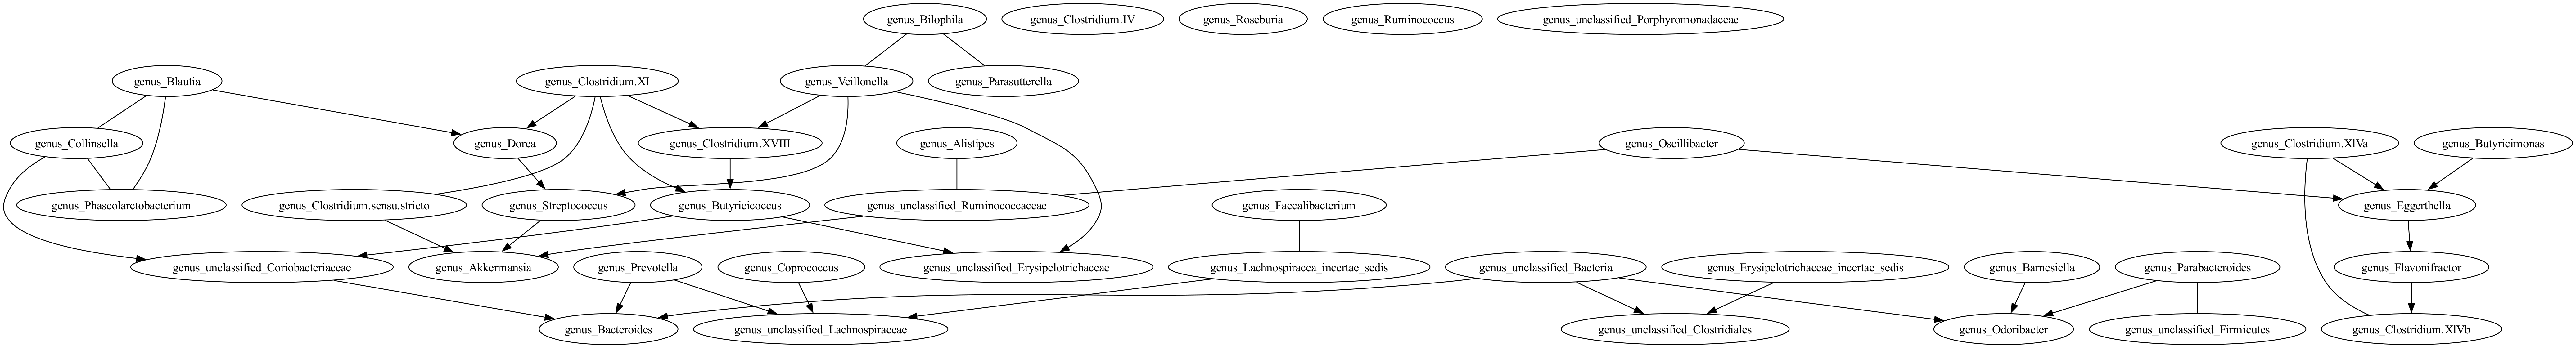
\includegraphics[width=\linewidth]{../graphs/t2d/sparcc_IS_norm.png}
  \caption{T2D Microbe-Microbe Network for IS after SparCC}
  \label{fig:t2dsparccISnorm}
\end{figure}

\begin{figure}[h!]
  \centering
  
\includegraphics[width=\linewidth]{../graphs/t2d/sparcc_IR_norm.png}
  \caption{T2D Microbe-Microbe Network for IR after SparCC}
  \label{fig:t2dsparccIRnorm}
\end{figure}

The microbe-microbe networks after SparCC for the two PCOS cohorts can be viewed on our website in higher resolution.

\clearpage
\textbf{Contributions}

MPM, CS, and NZ designed the project. MPM and CS found datasets. CS and NZ performed EDA. CS built the microbe-microbe and microbe-disease interaction networks. MPM built the VAE model. BH assisted in causal discovery methods and interpretation. JB proposed the feature reduction and sure screening methods. BH and JB provided insightful comments and suggestions to the design. MPM, CS, and NZ interpreted the results and wrote the final report. NZ built the website. MPM ran the upstream analysis using QIIME2. 

We thank Dr. Sam Degregori (Knight Lab) for guidance on BIRDMAn and the additional T2D meta-analysis studies. 


\end{document}